\documentclass[10pt]{beamer}

\usetheme{metropolis}
\usepackage[utf8]{inputenc}
\usepackage[brazilian]{babel}

\usepackage{booktabs}
\usepackage[scale=2]{ccicons}
\usepackage{listings}

\usepackage{pgfplots}
\usepgfplotslibrary{dateplot}

%Justificar texto
\usepackage{ragged2e}
\addtobeamertemplate{block begin}{}{\justifying}

\usepackage{xspace}
\newcommand{\themename}{\textbf{\textsc{metropolis}}\xspace}

\usepackage{tikz}
\usetikzlibrary{shapes,arrows}

\title{Projeto e Implementação em Controlador Industrial para Posicionamento de Risers com Validação Experimental}
%\subtitle{A modern beamer theme}
\date{\today}
\author{Ataias Pereira Reis\\ Emanuel Pereira Barroso Neto}
\institute{Faculdade de Tecnologia\\ Universidade de Brasília}
 \titlegraphic{\hfill
\includegraphics[height=1.0cm]{figures/logoVerdeUnB}}

\begin{document}

\maketitle

\begin{frame}{Índice}
  \setbeamertemplate{section in toc}[sections numbered]
  \tableofcontents[hideallsubsections]
\end{frame}

\section{Introdução}

\begin{frame}[fragile]{Risers}

\begin{columns}[T] % align columns
\begin{column}{.5\textwidth}
%\color{red}\rule{\linewidth}{4pt}

\begin{block}{} Há diversas operações realizadas em plataformas de petróleo em alto mar. Entre elas, a operação de reentrada dos risers. Este procedimento é muitas vezes realizado manualmente. A proposta deste trabalho é mostrar que é possível fazer isso de forma automática, por meio de testes em bancada laboratorial.\end{block}

\end{column}%
\hfill%
\begin{column}{.5\textwidth}
%\color{blue}\rule{\linewidth}{4pt}

\begin{figure}[!ht]
\centering
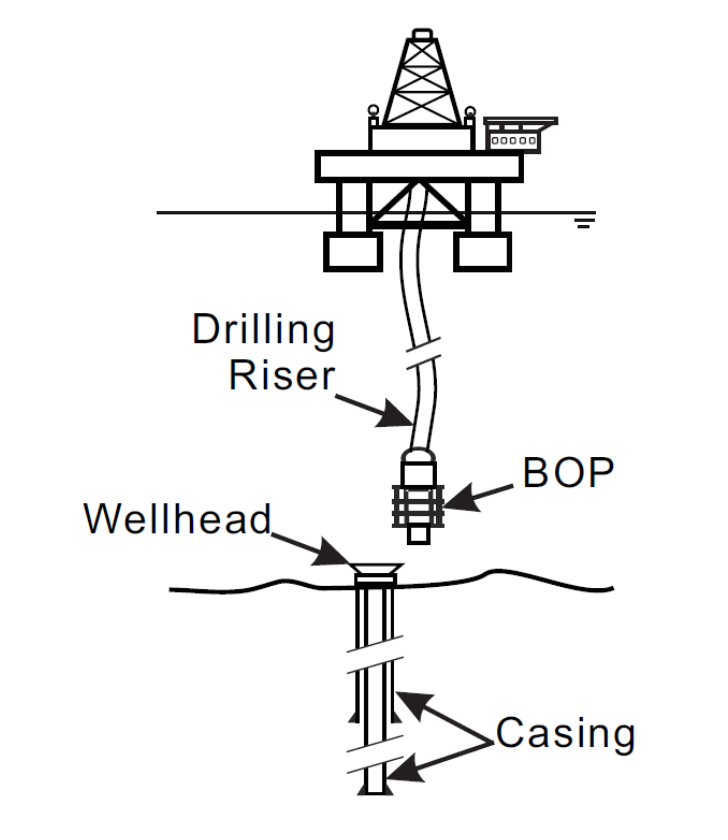
\includegraphics[width=1\linewidth]{figures/introducao/riser}
\caption{Operação de Reentrada \cite{redytton}}
\end{figure}

\end{column}%
\end{columns}

\end{frame}
\begin{frame}[fragile]{Risers}
  \begin{columns}[T] % align columns
\begin{column}{.5\textwidth}
%\color{red}\rule{\linewidth}{4pt}

\begin{figure}[!ht]
\centering
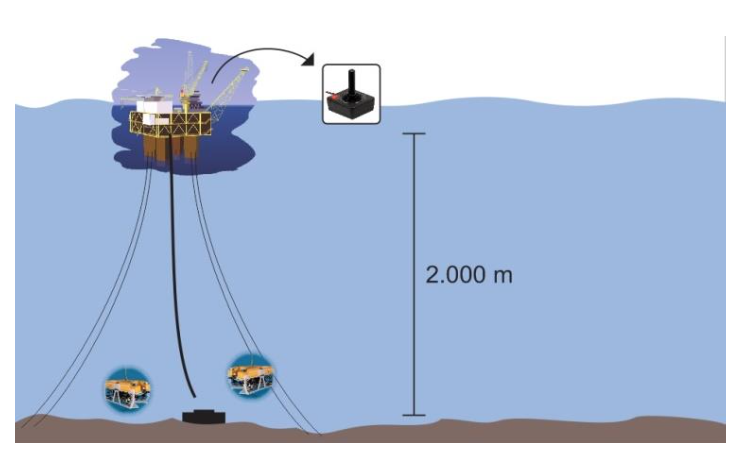
\includegraphics[width=1\linewidth]{figures/introducao/posicionamentoAtual}
\caption{Método atual para reconexão no poço \cite{redytton}}
\end{figure}


\end{column}%
\hfill%
\begin{column}{.5\textwidth}
%\color{blue}\rule{\linewidth}{4pt}

\begin{figure}[!ht]
\centering
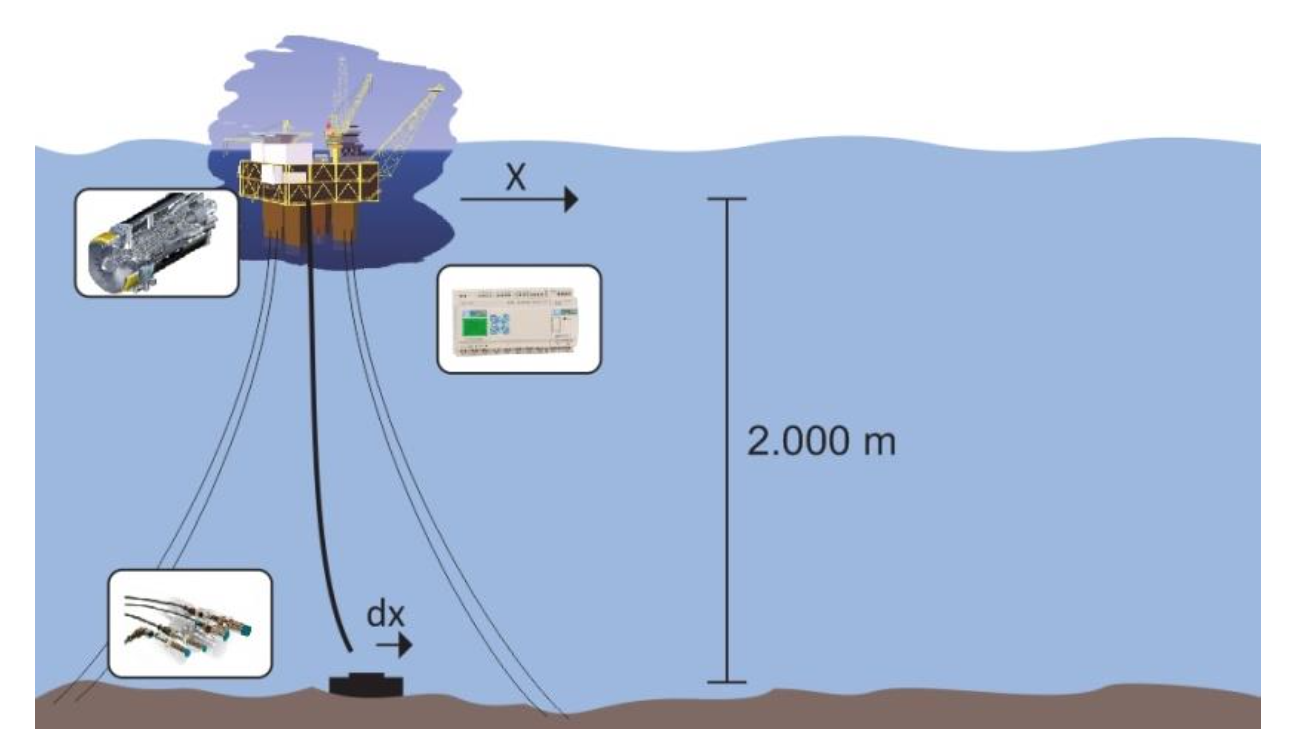
\includegraphics[width=1\linewidth]{figures/introducao/posicionamentoProposto}
\caption{Método proposto para reconexão no poço \cite{redytton}}
\end{figure}

\end{column}%
\end{columns}

\end{frame}

\section{Fundamentos}

\begin{frame}[fragile]{Equações Governantes}

\begin{block}{}
Utiliza-se a simplificação de Euler-Bernoulli para vigas, uma vez que \textit{risers} são esbeltos e possuem alto módulo de cisalhamento.
\end{block}

\begin{block}{}
A equação diferencial parcial para a variável deslocamento, $\Upsilon$, é dada por \begin{align}
	m_s \frac{\partial^2 \Upsilon}{\partial t^2} &= -E J	\frac{\partial^4 \Upsilon}{\partial z^4} + \frac{\partial}{\partial z}\left(T(z) \frac{\partial \Upsilon}{\partial z}\right) + F_n(z,t),
\end{align} na qual $m_s$ é a densidade linear do tubo, $E$ é o módulo de Young e $J$ é o segundo momento de inércia do \textit{riser}. $T(z)$ descreve as forças de tração ao longo do comprimento do \textit{riser}. $F_n(z,t)$ é a força resultante externa \cite{fabricioIFAC}.
\end{block}

\end{frame}

\begin{frame}[fragile]{Controle - Malha Aberta x Malha Fechada}

\tikzstyle{block} = [draw, fill=blue!20, rectangle,font=\tiny, 
minimum height=0.5em, minimum width=1em]
\tikzstyle{sum} = [draw, fill=blue!20, circle, node distance=1cm]
\tikzstyle{input} = [coordinate]
\tikzstyle{output} = [coordinate]
\tikzstyle{pinstyle} = [pin edge={to-,thin,black}]

\begin{columns}[T,onlytextwidth]

\begin{column}{.5\textwidth}

\begin{figure}[!ht]
	
	%\centering
	% The block diagram code is probably more verbose than necessary
	\begin{tikzpicture}[auto, node distance=1cm,>=latex']
	% We start by placing the blocks
	\node [input, name=input] {};
	\node [block, right of=input] (controller) {Controlador};
	\node [block, right of=controller, pin={[pinstyle,font=\small]above:Perturbações},
	node distance=2cm] (system) {Planta};
	% We draw an edge between the controller and system block to 
	% calculate the coordinate u. We need it to place the measurement block. 
	\draw [->] (controller) -- node[name=u] {$u$} (system);
	\node [output, right of=system] (output) {};
	
	% Once the nodes are placed, connecting them is easy. 
	\draw [draw,->] (input) -- node {$r$} (controller);
	\draw [->] (system) -- node [name=y] {$y$}(output); 
	\end{tikzpicture}
	\caption{Malha aberta de controle\label{mabertatikz}}
\end{figure}


\begin{figure}[!ht]
\centering
% The block diagram code is probably more verbose than necessary

\begin{tikzpicture}[auto, node distance=1cm,>=latex']
% We start by placing the blocks
\node [input, name=input] {};
\node [sum, right of=input] (sum) {};
\node [block, right of=sum] (controller) {Controlador};
\node [block, right of=controller, pin={[pinstyle,font=\small]above:Perturbações},
node distance=1.5cm] (system) {Planta};
% We draw an edge between the controller and system block to 
% calculate the coordinate u. We need it to place the measurement block. 
\draw [->] (controller) -- node[name=u] {$u$} (system);
\node [output, right of=system] (output) {};
\node [block, below of=u] (measurements) {Medição};

% Once the nodes are placed, connecting them is easy. 
\draw [draw,->] (input) -- node {$r$} (sum);
\draw [->] (sum) -- node {$e$} (controller);
\draw [->] (system) -- node [name=y] {$y$}(output);
\draw [->] (y) |- (measurements);
\draw [->] (measurements) -| node[pos=0.99] {$-$} 
node [near end] {$y_m$} (sum);
\end{tikzpicture}
\caption{Malha fechada de controle\label{mfechadatikz}}
\end{figure}
\end{column}

\begin{column}{.5\textwidth}

\begin{block}{Controle em Malha Aberta}
Saída não é realimentada - não necessita do uso de sensores.
\newline
\newline
\newline
\end{block}

\begin{block}{Controle em Malha Fechada}
Possui realimentação - obtém o sinal de referência para a planta pela evolução do erro.\end{block}

\end{column}

\end{columns}
\end{frame}

\begin{frame}[fragile]{Bancada - Esquemático}
\begin{figure}[!ht]
	\centering
	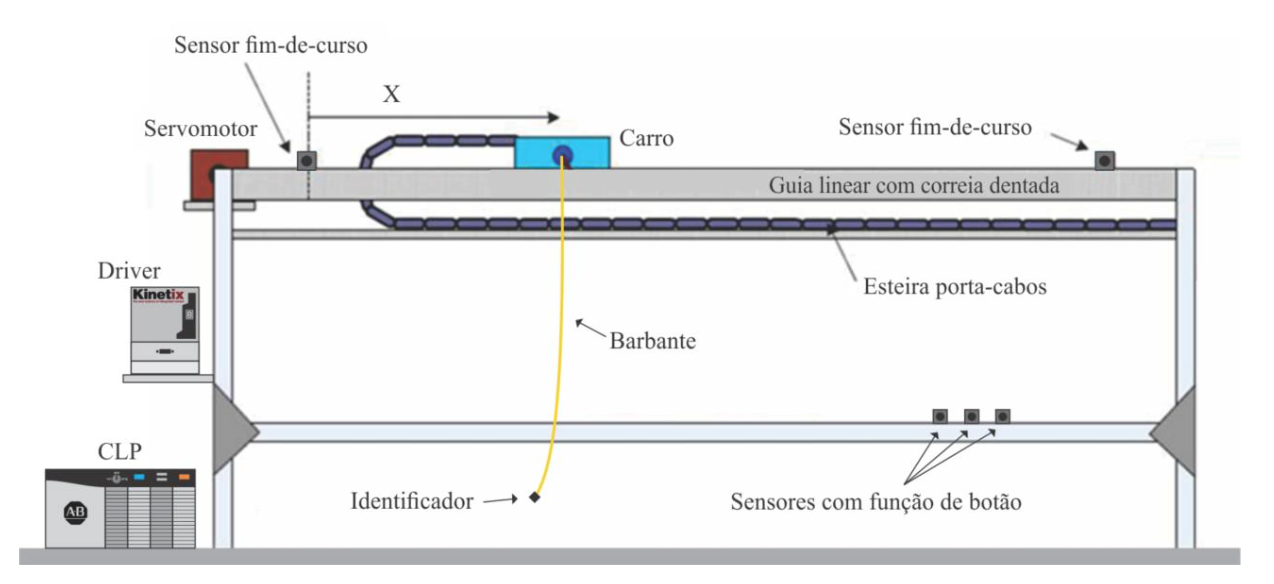
\includegraphics[width=.9\linewidth]{figures/fundamentos/bancadaEsquematico}
	\caption{Esquemático da ponte rolante \cite{redytton}}
	\label{bancadaesq}
\end{figure}
\end{frame}

\begin{frame}[fragile]{Bancada - Controlador}
\begin{block}{}
Responsável por receber dados da câmera e dos sensores, processá-los e enviar sinais de controle para o motor.
\end{block}
\begin{figure}[!ht]
	\centering
	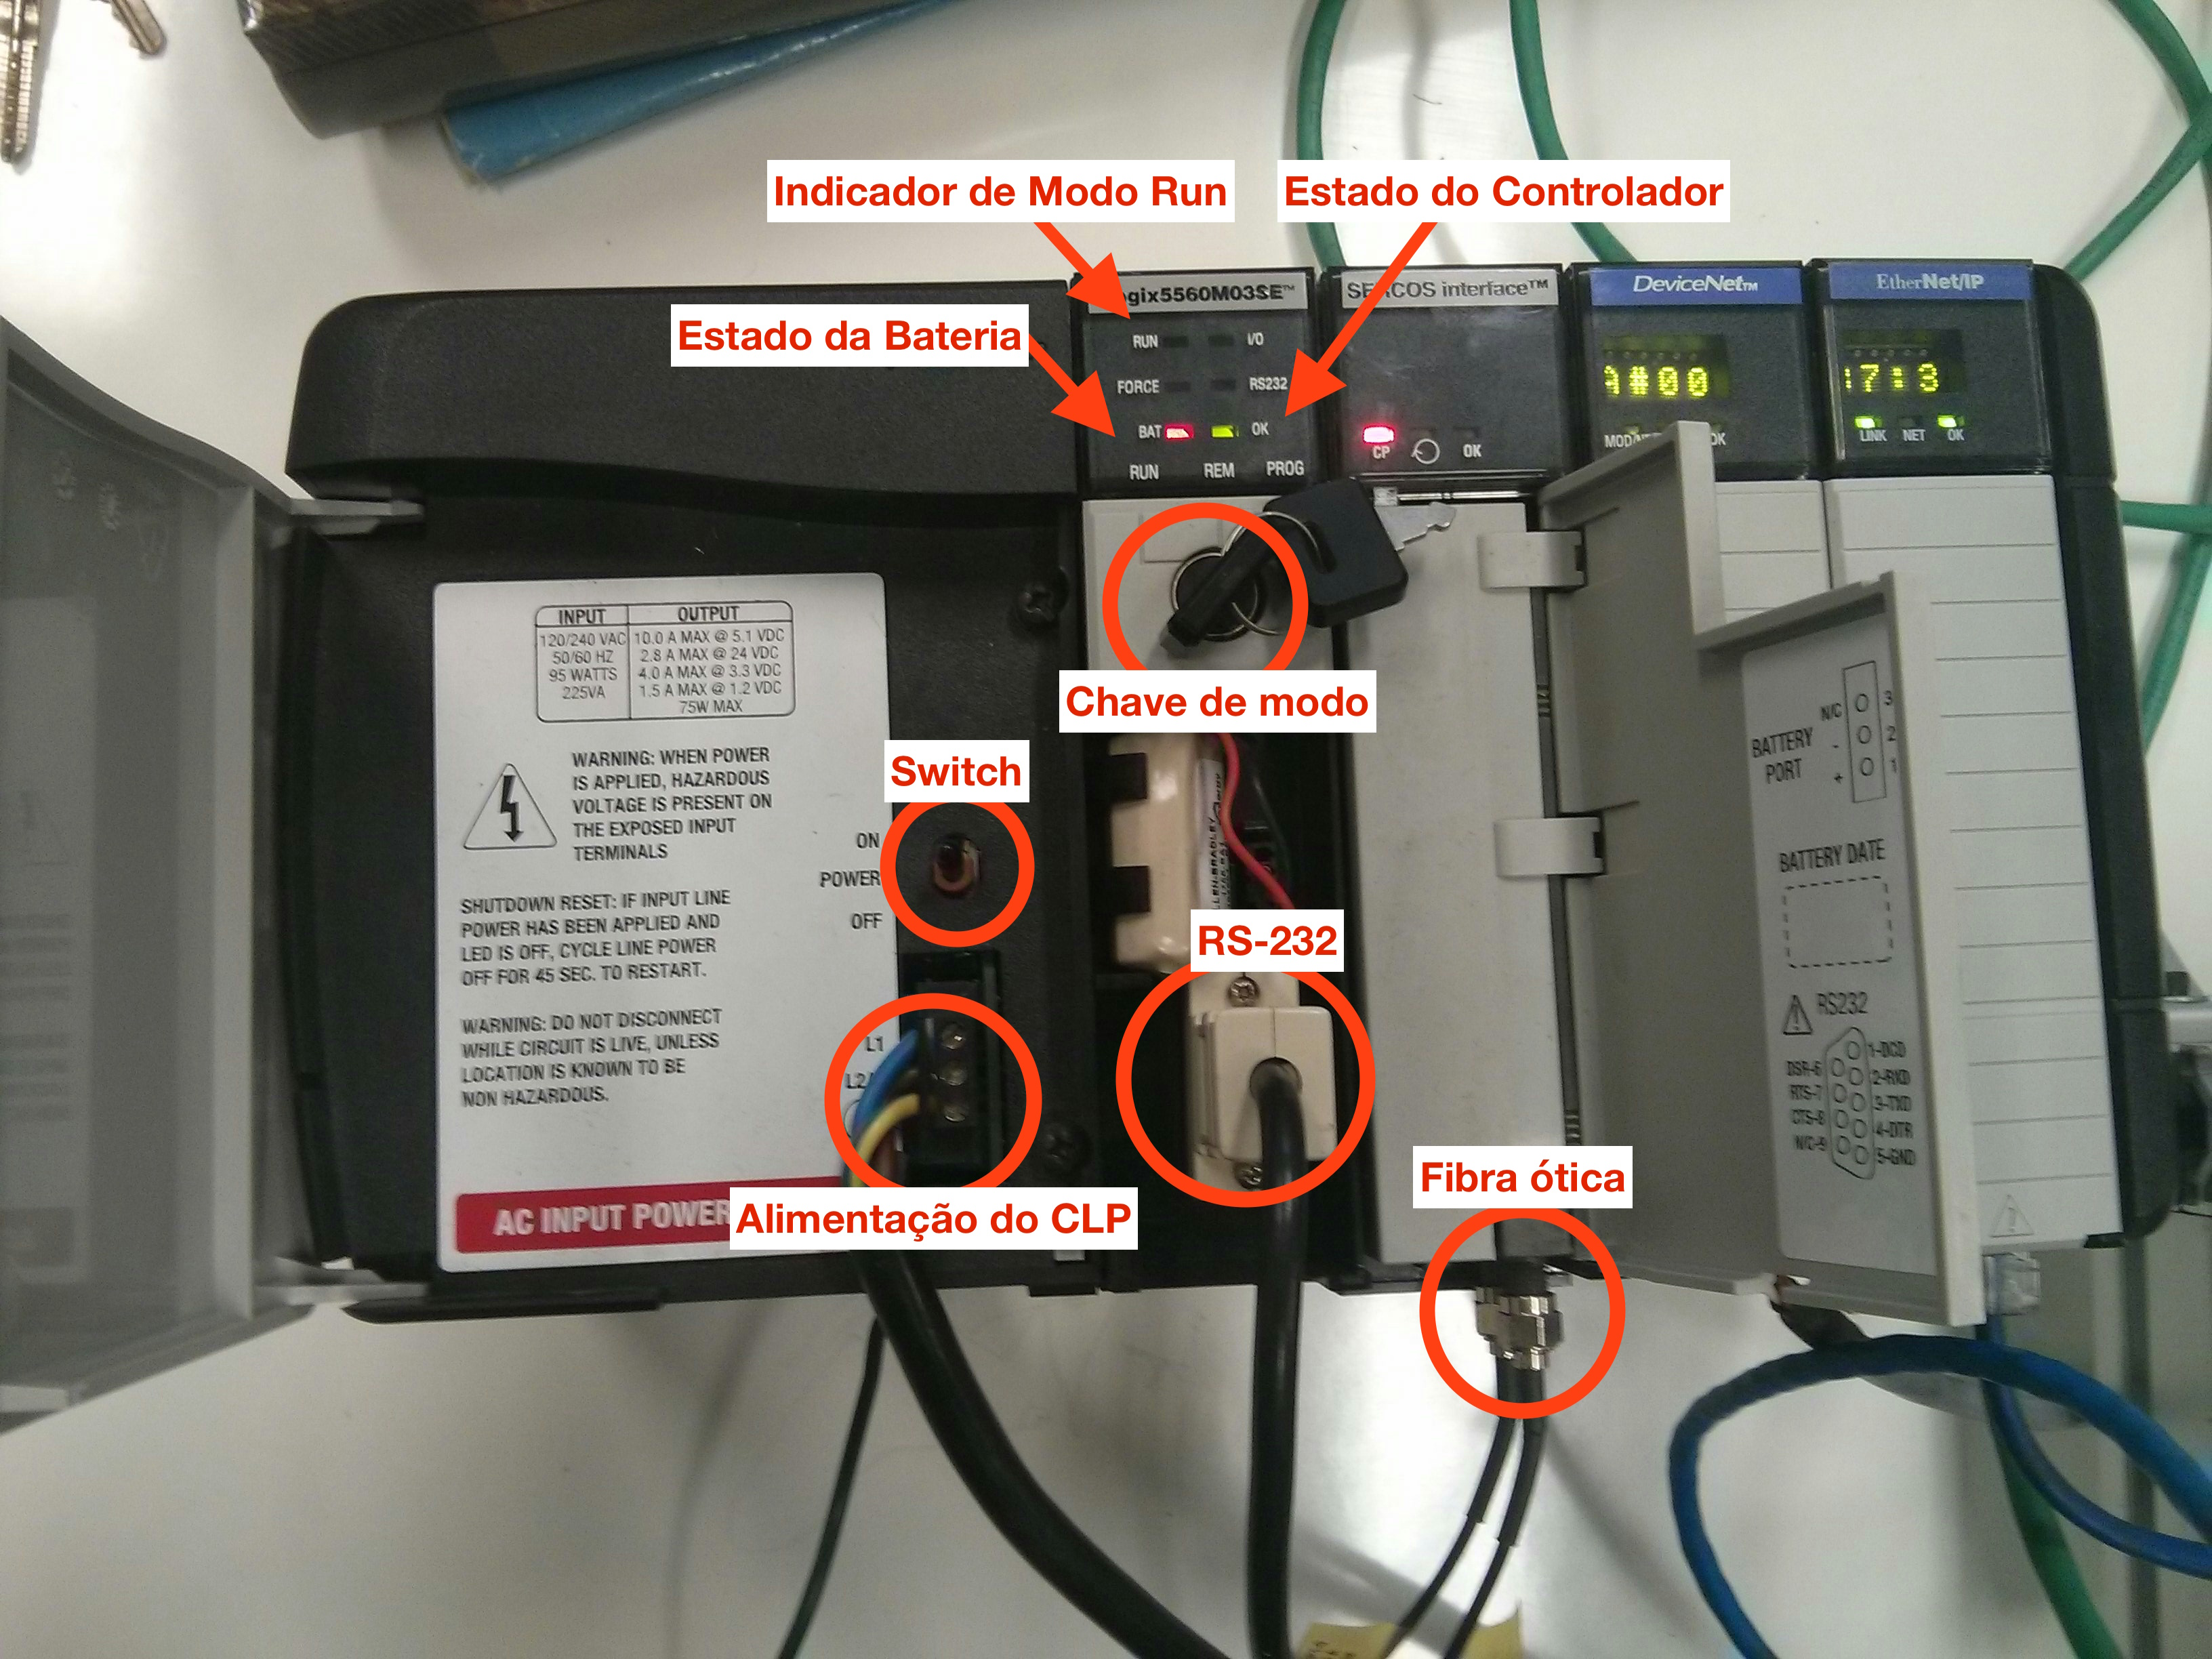
\includegraphics[width=.6\linewidth]{figures/fundamentos/CLP}
	\caption{Controlador Lógico Programável da \textit{Allen-Bradley}}
	\label{clpfig}
\end{figure}
\end{frame}

\begin{frame}[fragile]{Bancada - Câmera e Drive Kinetix}
\begin{columns}[T]

\begin{column}{.5\textwidth}
\begin{block}{Câmera}
Responsável por enviar a posição da bolinha para o CLP. Atua como sensor visual.
\end{block}

\begin{figure}[!ht]
	\centering
	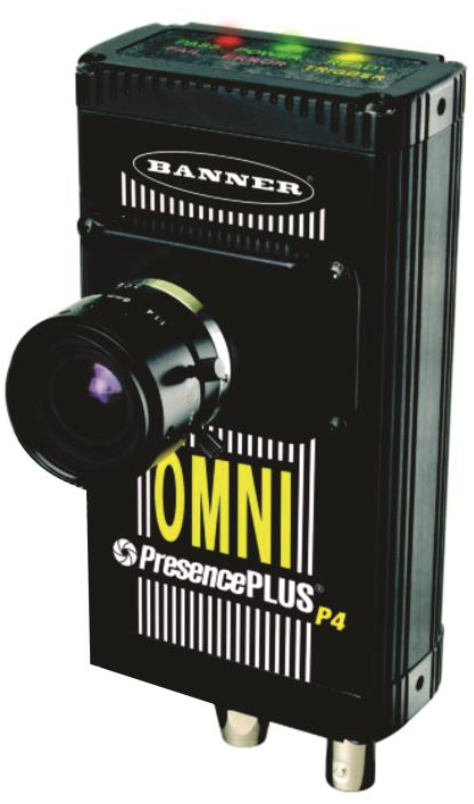
\includegraphics[width=.3\linewidth]{figures/fundamentos/camera}
	\caption{Câmera \textit{Presence Plus} \cite{redytton}}
	\label{bancadacamera}
\end{figure}

\end{column}

\begin{column}{.5\textwidth}

\begin{block}{Drive Kinetix}
Responsável por fornecer potência para o motor e controlá-lo por meio de pulsos PWM.
\end{block}

\begin{figure}[!ht]
	\centering
	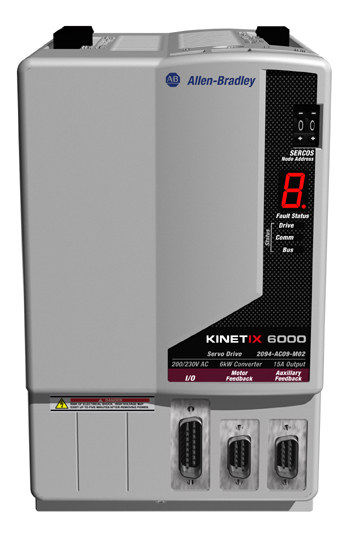
\includegraphics[width=.3\linewidth]{figures/fundamentos/kinetix6000}
	\caption{\textit{Drive Kinetix 6000} \cite{redytton}}
	\label{bancadadrive}
\end{figure}

\end{column}

\end{columns}
\end{frame}

\begin{frame}[fragile]{Bancada - \textit{Line Interface Module}}
\begin{block}{}
Responsável pela interface elétrica entre o \textit{Drive Kinetix} e a rede de alimentação trifásica.
\end{block}

\begin{figure}[!ht]
	\centering
	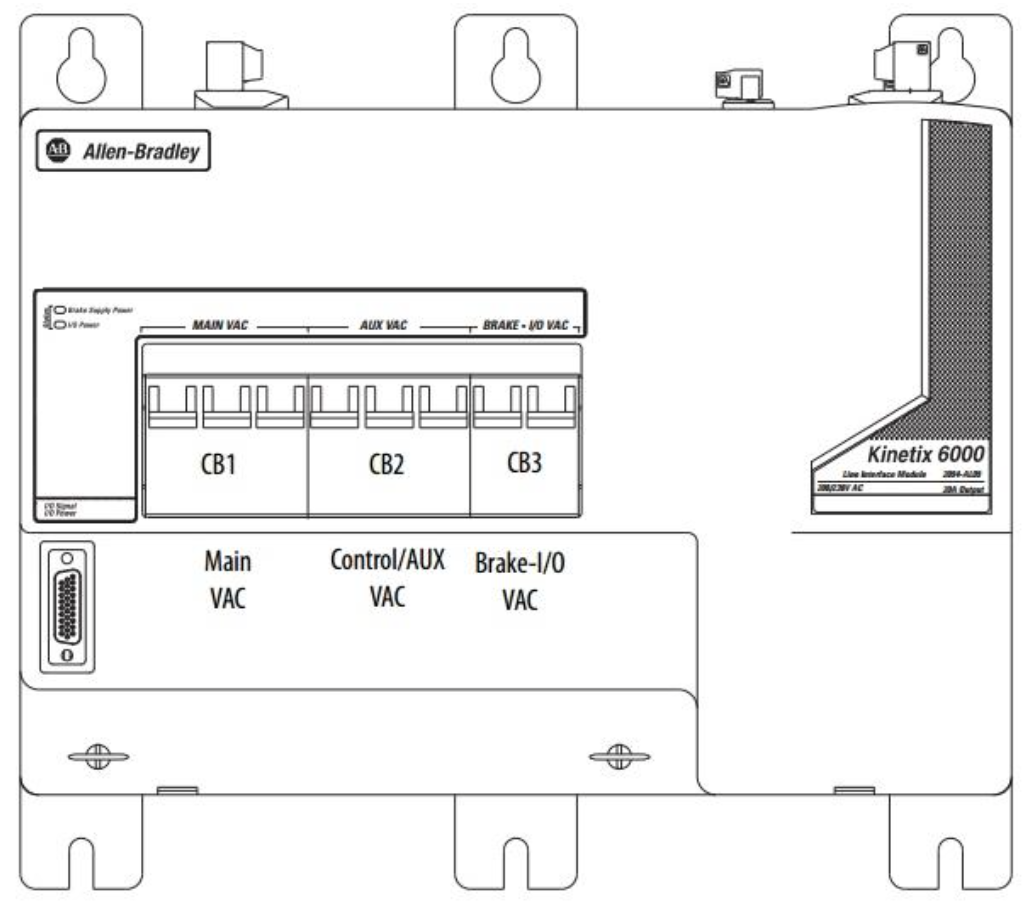
\includegraphics[width=.5\linewidth]{figures/fundamentos/LineInterfaceModule}
	\caption{\textit{Line Interface Module} \cite{redytton}}
	\label{bancadalim}
\end{figure}

\end{frame}

\begin{frame}[fragile]{Bancada - Sensores Indutivos e Servomotor}

\begin{columns}[T]

\begin{column}{.5\textwidth}

\begin{block}{Sensores Indutivos}
Detectam objetos metálicos; podem operar em modo analógico ou digital. Utilizados como chaves de fim de curso para a rotina de emergência.
\end{block}

\begin{figure}[!ht]
	\centering
	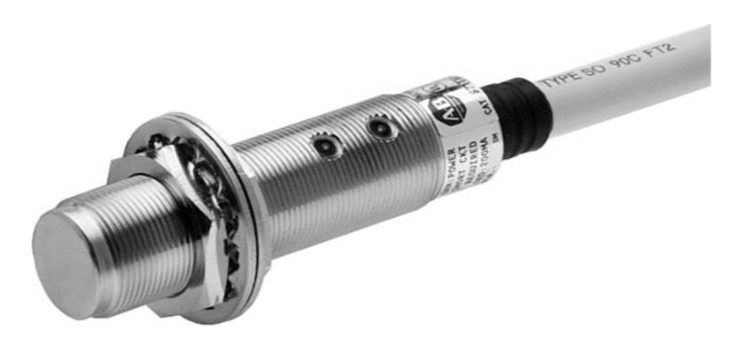
\includegraphics[width=.6\linewidth]{figures/fundamentos/sensorIndutivo}
	\caption{Sensor Indutivo \cite{redytton}}
	\label{bancadaindut}
\end{figure}

\end{column}

\begin{column}{.5\textwidth}

\begin{block}{Servomotor}
Atuador rotatório composto de motor elétrico com sensor acoplado; permite controle preciso da posição angular.
\end{block}

\begin{figure}[!ht]
	\centering
	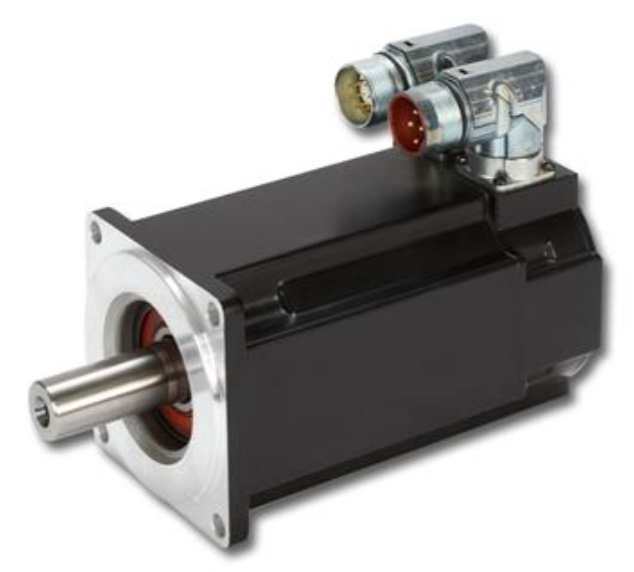
\includegraphics[width=.5\linewidth]{figures/fundamentos/servomotor}
	\caption{Servomotor \cite{redytton}}
	\label{bancadaservo}
\end{figure}

\end{column}

\end{columns}

\end{frame}

\begin{frame}[fragile]{Redes Industriais}
\begin{columns}[T]
\begin{column}{.5\textwidth}
\begin{block}{DeviceNet}
Rede responsável por conectar os sensores indutivos ao CLP por meio do módulo 1756-DNB. Suporta conexões de dispositivos de baixo nível com CLPs e outros dispositivos de alto nível, como o computador \cite{devicenetrockwell}. O módulo responsável pelo \textit{scan} desta rede é o \textit{1756-DNB}.
\end{block}
\end{column}

\begin{column}{.5\textwidth}
\begin{block}{Ethernet/IP}
Transmite dados da câmera para o CLP, e também transfere os programas em \textit{ladder} ou texto estruturado do computador para o controlador. É uma rede indicada para aplicações em que o tempo é crítico \cite{eiprockwell}. O módulo responsável pelo \textit{scan} desta rede é o \textit{1756-ENBT/A}.
\end{block}
\end{column}

\end{columns}
\end{frame}

\begin{frame}[fragile]{Programação CLP - Passos}
\begin{block}{Passos para programação em CLP}
\begin{enumerate}
  \item Descrição do problema;
  \item Detalhamentos e melhoria do processo;
  \item Especificação dos atuadores e sensores da planta;
  \item Elaboração do algoritmo;
  \item Representação gráfica do algoritmo, quando aplicável;
  \item Esquema funcional, quando aplicável;
  \item Seleção dos módulos do controlador;
  \item Programação, utilizando linguagens suportadas.
\end{enumerate}
\end{block}
\end{frame}

\begin{frame}[fragile]{Linguagem \textit{Ladder}}
\begin{block}{}
Linguagem gráfica para CLPs. Lembra conexões elétricas de sistemas com relés.

\begin{figure}[!ht]
	\centering
	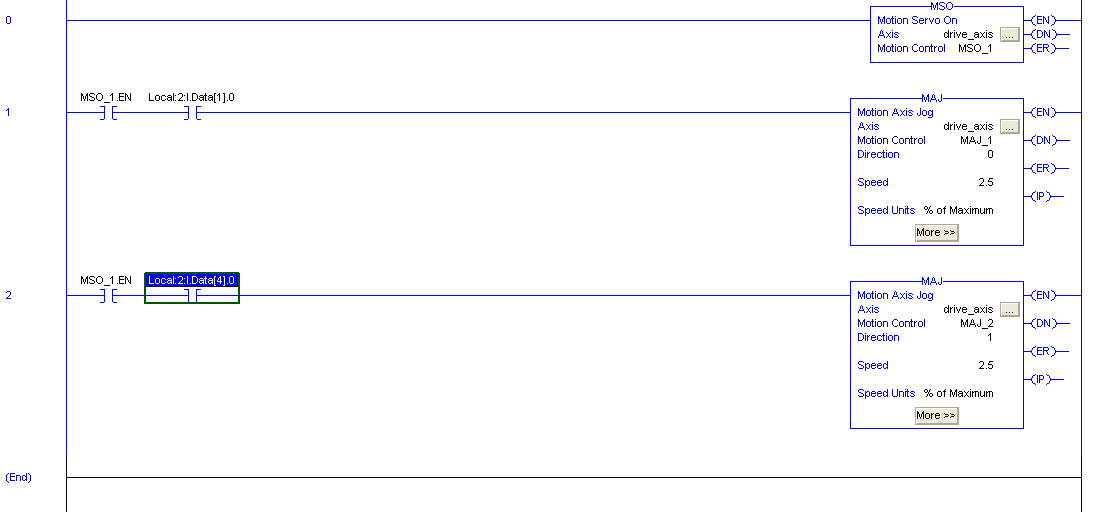
\includegraphics[width=.9\linewidth]{figures/fundamentos/motionladder}
	\caption{Exemplo de programa em \textit{ladder}}
	\label{laddersample}
\end{figure}
\end{block}
\end{frame}

\begin{frame}[fragile]{Texto Estruturado}

\begin{columns}[T]

\begin{column}{.5\textwidth}
\begin{block}{Texto Estruturado}
Linguagem sequencial, semelhante a linguagens como C ou Pascal. Os comandos são executados em sequência, de cima para baixo.
\end{block}
\end{column}

\begin{column}{.5\textwidth}
\lstinputlisting{codes/sample.txt}
\end{column}

\end{columns}

\end{frame}

\begin{frame}[fragile]{Parâmetros Para Geração de Trajetórias}
\begin{table}[!ht]
\centering
\caption{Dados para simulação em escala real\label{escalaReal} \cite{redytton}}
	\begin{tabular}{|c|c|}
	\hline
		\multicolumn{2}{|c|}{\textbf{Dados do Riser}}\\ \hline
		Diâmetro externo & $0.55\mathrm{m}$\\ \hline
		Diâmetro interno & $0.5\mathrm{m}$ \\ \hline
		Comprimento & $2000\mathrm{m}$ \\ \hline
		Módulo de Elasticidade & $200 \mathrm{GPa}$\\ \hline
		Densidade &  $7860\mathrm{kg}/\mathrm{m}^3$\\ \hline
		\multicolumn{2}{|c|}{\textbf{Dados do fluido (Água)}}\\ \hline
		Densidade do fluido &  $1000\mathrm{kg}/\mathrm{m}^3$\\ \hline
		Viscosidade dinâmica & $10^3 \mathrm{Pa}\cdot \mathrm{s}$ \\ \hline
	\end{tabular}



\end{table}

\end{frame}

\begin{frame}[fragile]{Parâmetros Para Geração de Trajetórias}

\begin{table}[!ht]
	\caption{Dados para simulação em escala laboratorial\label{escalaLaboratorial}}
	\centering
	\begin{tabular}{|c|c|}
		\hline
			\multicolumn{2}{|c|}{\textbf{Dados da Massa na Ponta - Isopor}} \\ \hline
			Diâmetro Externo & $30.6\mathrm{mm}$\\ \hline
			Densidade & $10\mathrm{kg}/\mathrm{m}^3$ \\ \hline
			\multicolumn{2}{|c|}{\textbf{Dados do Riser (Barbante)}}\\ \hline
			Diâmetro externo & $2\mathrm{mm}$\\ \hline
			Diâmetro interno & $0\mathrm{mm}$ \\ \hline
			Comprimento & $82\mathrm{cm}$ \\ \hline
			Módulo de Elasticidade & $2.1 \mathrm{MPa}$\\ \hline
			Densidade &  $191\mathrm{kg}/\mathrm{m}^3$\\ \hline
			\multicolumn{2}{|c|}{\textbf{Dados do fluido (Ar)}}\\ \hline
			Densidade do fluido &  $1.2754\mathrm{kg}/\mathrm{m}^3$\\ \hline
			Viscosidade dinâmica & $17.2\cdot 10^6 \mathrm{Pa}\cdot \mathrm{s}$ \\ \hline
		\end{tabular}
\end{table}

\end{frame}
%{
%\metroset{titleformat frame=smallcaps}
%\begin{frame}{Small caps}
%	This frame uses the \texttt{smallcaps} titleformat.
%
%	\begin{alertblock}{Potential Problems}
%		Be aware, that not every font supports small caps. If for example you typeset your presentation with pdfTeX and the Computer Modern Sans Serif font, every text in smallcaps will be typeset with the Computer Modern Serif font instead.
%	\end{alertblock}
%\end{frame}
%}
%
%{
%\metroset{titleformat frame=allsmallcaps}
%\begin{frame}{All small caps}
%	This frame uses the \texttt{allsmallcaps} titleformat.
%
%	\begin{alertblock}{Potential problems}
%		As this titleformat also uses smallcaps you face the same problems as with the \texttt{smallcaps} titleformat. Additionally this format can cause some other problems. Please refer to the documentation if you consider using it.
%
%		As a rule of thumb: Just use it for plaintext-only titles.
%	\end{alertblock}
%\end{frame}
%}
%
%{
%\metroset{titleformat frame=allcaps}
%\begin{frame}{All caps}
%	This frame uses the \texttt{allcaps} titleformat.
%
%	\begin{alertblock}{Potential Problems}
%		This titleformat is not as problematic as the \texttt{allsmallcaps} format, but basically suffers from the same deficiencies. So please have a look at the documentation if you want to use it.
%	\end{alertblock}
%\end{frame}
%}

\section{Resultados}

\begin{frame}[fragile]{Calibração da Câmera}
\begin{block}{Passos para a calibração da câmera}
\begin{enumerate}
	\item Atualização do \textit{firmware};
	\item Reconhecimento da câmera pelo \textit{software RsLinx};
	\item Estabelecimento de um endereço IP para a câmera no \textit{software PresencePlus};
	\item Uso das ferramentas de tomada de dados da câmera no \textit{software PresencePlus};
	\item Obtenção da relação entre \textit{pixels} da câmera e milímetros.
\end{enumerate}
\end{block}
\end{frame}

\begin{frame}[fragile]{Calibração da Câmera}
\begin{block}{Ferramentas utilizadas}
\begin{itemize}
	\item \texttt{Locate}: Localiza o corpo desejado pelas bordas;
	\item \texttt{Geometric}: Localiza o ``centro geométrico'' do corpo a ser detectado;
	\item \texttt{Measure}: Responsável por efetuar medições em \textit{pixels} entre pontos de referência desejados;
	\item \texttt{Math}: Executa cálculos matemáticos;
	\item \texttt{Communication}: Transfere os dados de interesse da câmera para o CLP por meio da rede Ethernet/IP.
\end{itemize}
\end{block}
\end{frame}

\begin{frame}[fragile]{Calibração da Câmera - Reconhecimento do \textit{Software RSLinx}}
\begin{figure}[!ht]
\centering
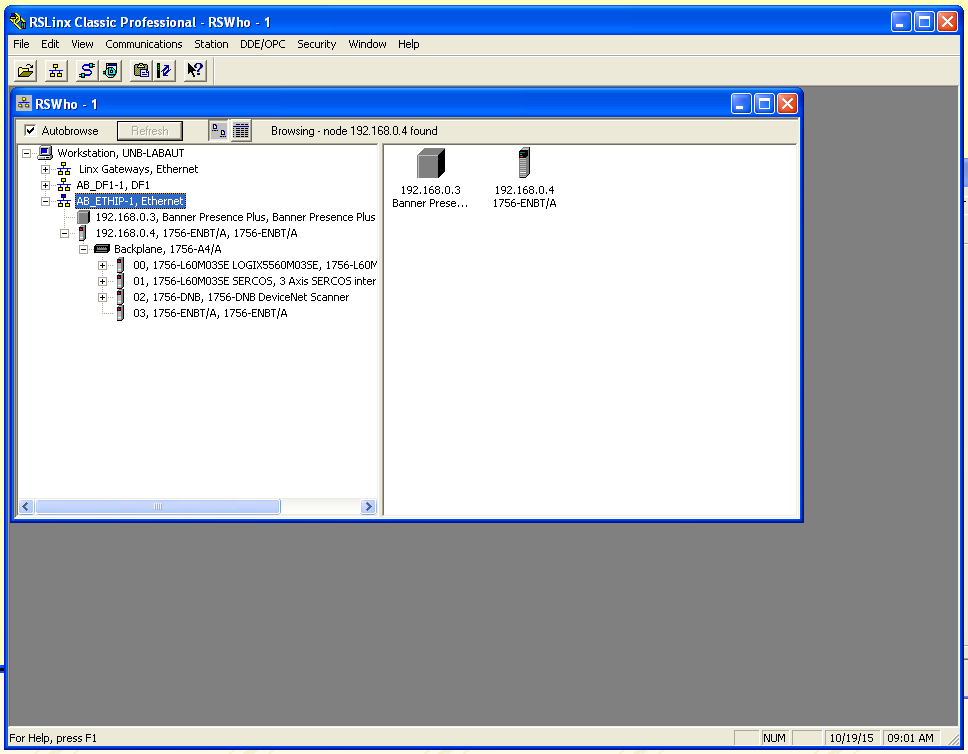
\includegraphics[width=.7\linewidth]{figures/resultados/camera/cameralinx}
\caption{\textit{RSLinx} com câmera reconhecida \label{linxcamera}}
\end{figure}
\end{frame}

\begin{frame}[fragile]{Calibração da Câmera - Configuração do Módulo Ethernet/IP}
\begin{figure}[!ht]
\centering
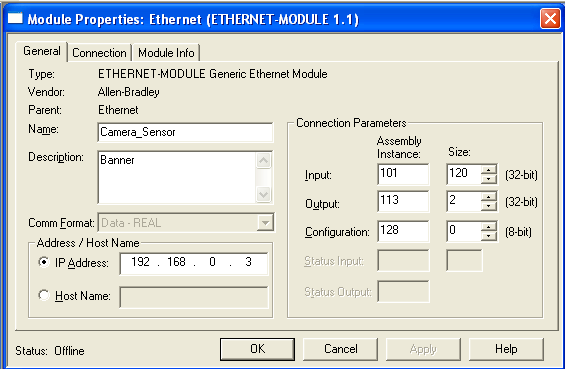
\includegraphics[width=.8\linewidth]{figures/resultados/camera/cameraSetup}
\caption{Configuração do módulo 1756-ENBT para uso dos dados da câmera\label{setupcamera}}
\end{figure}
\end{frame}

\begin{frame}[fragile]{Calibração da Câmera - \textit{Software PresencePlus}}
\begin{figure}[!ht]
\centering
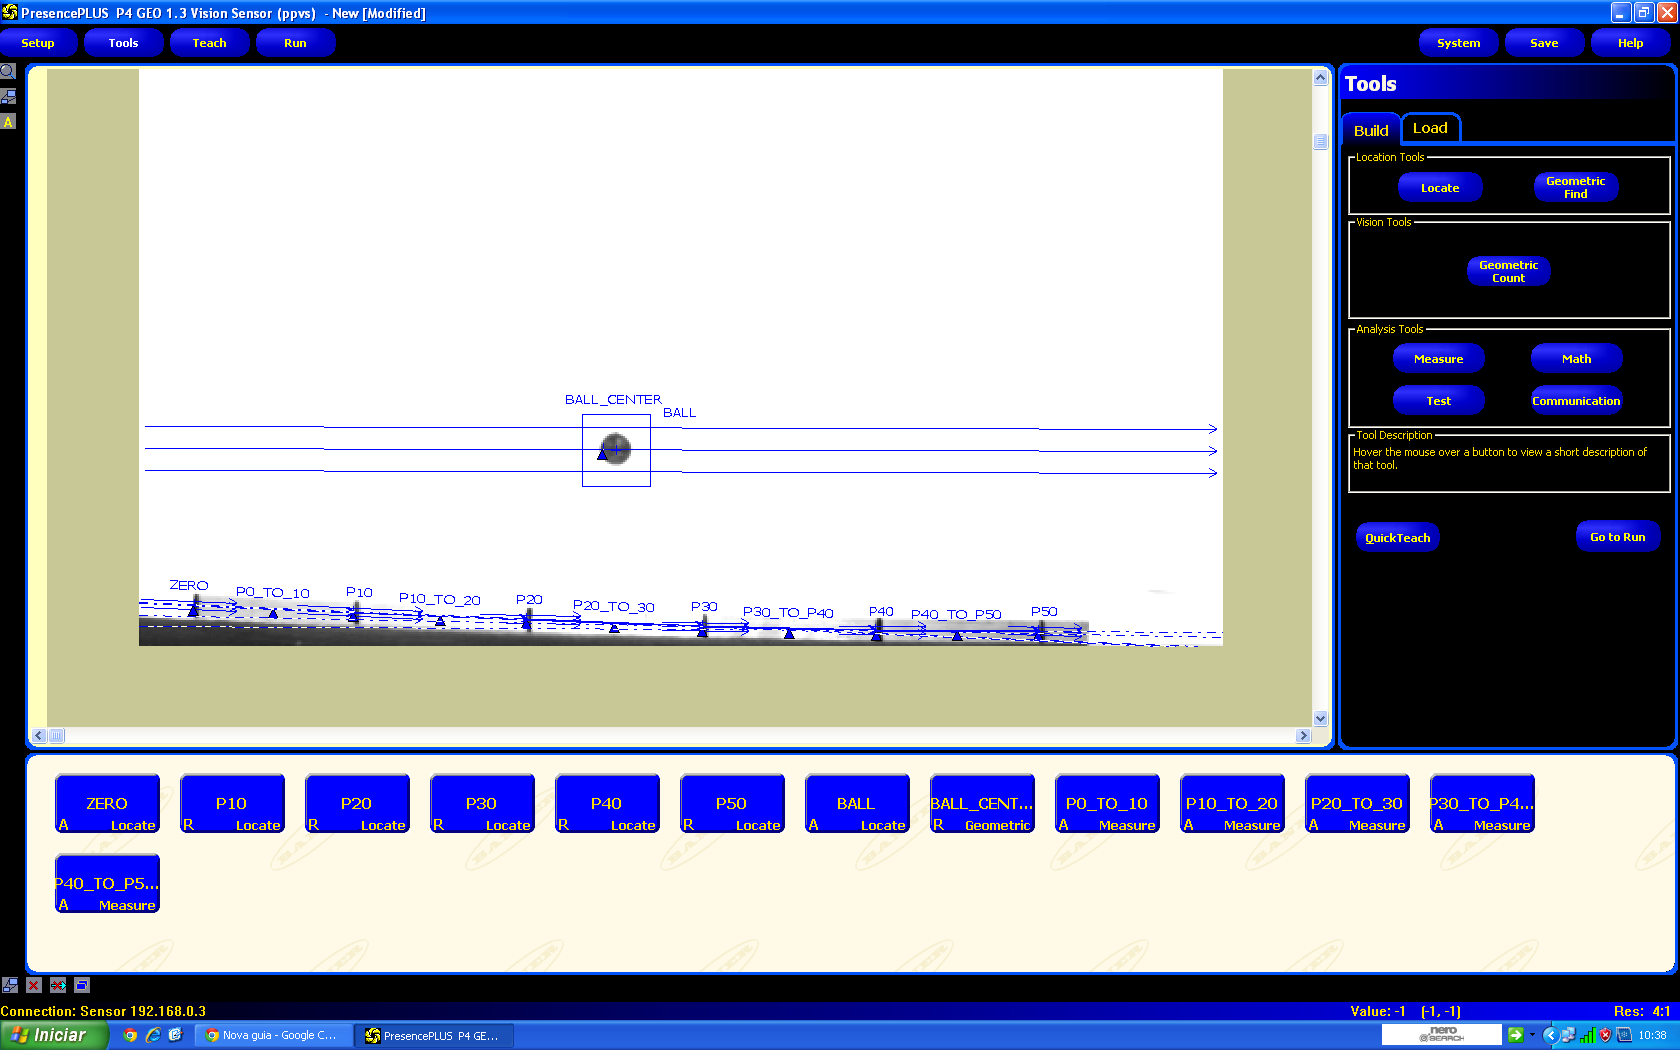
\includegraphics[width=.9\linewidth]{figures/resultados/camera/programa}
\caption{Calibração da câmera pelo \textit{software PresencePlus} \label{calibcamera}}
\end{figure}
\end{frame}

\begin{frame}[fragile]{Calibração da Câmera - Resultados}
\begin{table}[!ht]
\centering
\caption{Relações mm/px para diferentes seções da barra de alumínio \label{relacoesmmpx}}
	\begin{tabular}{|c|c|c|c|}
	\hline
		Seção 1 & Seção 2 & Distância (px) & mm/px\\ \hline
		P0 & P10 & 160 & 0.625\\ \hline
		P10 & P20 & 173 & 0.578\\ \hline
		P20 & P30 & 176 & 0.568\\ \hline
		P30 & P40 & 173 & 0.578\\ \hline
		P40 & P50 & 163 & 0.613\\ \hline
		P0 & PEND & 893 & 0.596\\ \hline
	\end{tabular}
\end{table}
Erro aproximado: 4.93 \%
\end{frame}

\begin{frame}[fragile]{Calibração do Servomotor}
\begin{block}{Passos para a calibração}
\begin{enumerate}
	\item Obtenção da posição inicial $x_0$ e posição final $x_f$, em milímetros;
	\item Definição de um intervalo de tempo $\Delta t$ e uma velocidade de movimentação do carrinho $v$ em $[\mathrm{u}/\mathrm{s}]$;
	\item Cálculo da velocidade em $[\mathrm{mm}/\mathrm{s}]$ a partir dos dados obtidos.
\end{enumerate}
\end{block}
\end{frame}

\begin{frame}[fragile]{Calibração do Servomotor - Resultados}

\begin{table}[!ht]
\centering
\caption{Dados de calibração do servomotor, média obtida é de 71.32 mm/unidade\label{calibracaoServomotor}}
\resizebox{\textwidth}{!}{
\begin{tabular}{|c|c|c|c|c|c|}
\hline
	$x_0$ - [mm] & $x_f$ - [mm] & $\Delta t$ - [s] & Velocidade - [u/s] & Velocidade - [mm/s] & mm/u\\ \hline
2 &	71.8  &	2   &	0.5 &	34.9   & 	69.8\\ \hline
6 & 76.1  &	2   &	0.5 &	35.05  &	70.1\\ \hline
6 &	188	  &  5   &	0.5	&   36.4   &	72.8\\ \hline
6 &	185   &	2.5 &	1	& 	71.6   &	71.6\\ \hline
6 &	77    &	10  &	0.1	&   7.1    &	71\\ \hline
6 &	296.5 &	20	&   0.2 & 	14.525 &	72.625\\ \hline\end{tabular}
}
\end{table}

\end{frame}

\begin{frame}[fragile]{Malha Aberta - Resultados}
\begin{block}{Excursão de 30 cm - Dados}
\begin{itemize}
	\item \textbf{Período de amostragem: } $T \approx 41 \mathrm{ms}$;
	\item \textbf{Deslocamento: } $\Delta x = 30 \mathrm{cm}$;
	\item \textbf{Intervalo de tempo: } $\Delta t \approx 3 \mathrm{s}$;
	\item \textbf{Velocidade média: } $\overline{v} = \frac{\Delta x}{\Delta t} = 100\mathrm{mm}/\mathrm{s}$.
	
\end{itemize}
\end{block}
\end{frame}

\begin{frame}[fragile]{Malha Aberta - Resultados}
\begin{block}{Excursão de 30 cm - Trajetória modelada}

\begin{figure}[!htb]
    \centering
    \begin{minipage}{.45\textwidth}
        \centering
        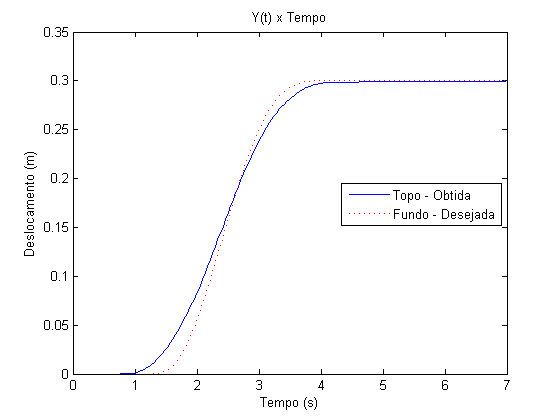
\includegraphics[width=1\linewidth]{figures/resultados/malha_aberta_1/DeslocamentoT1}
        \caption{Referência de Posição para Excursão de 30cm}
        \label{DeslocamentoT1}
    \end{minipage}%
    \hspace{0.1cm}
    \begin{minipage}{0.45\textwidth}
        \centering
        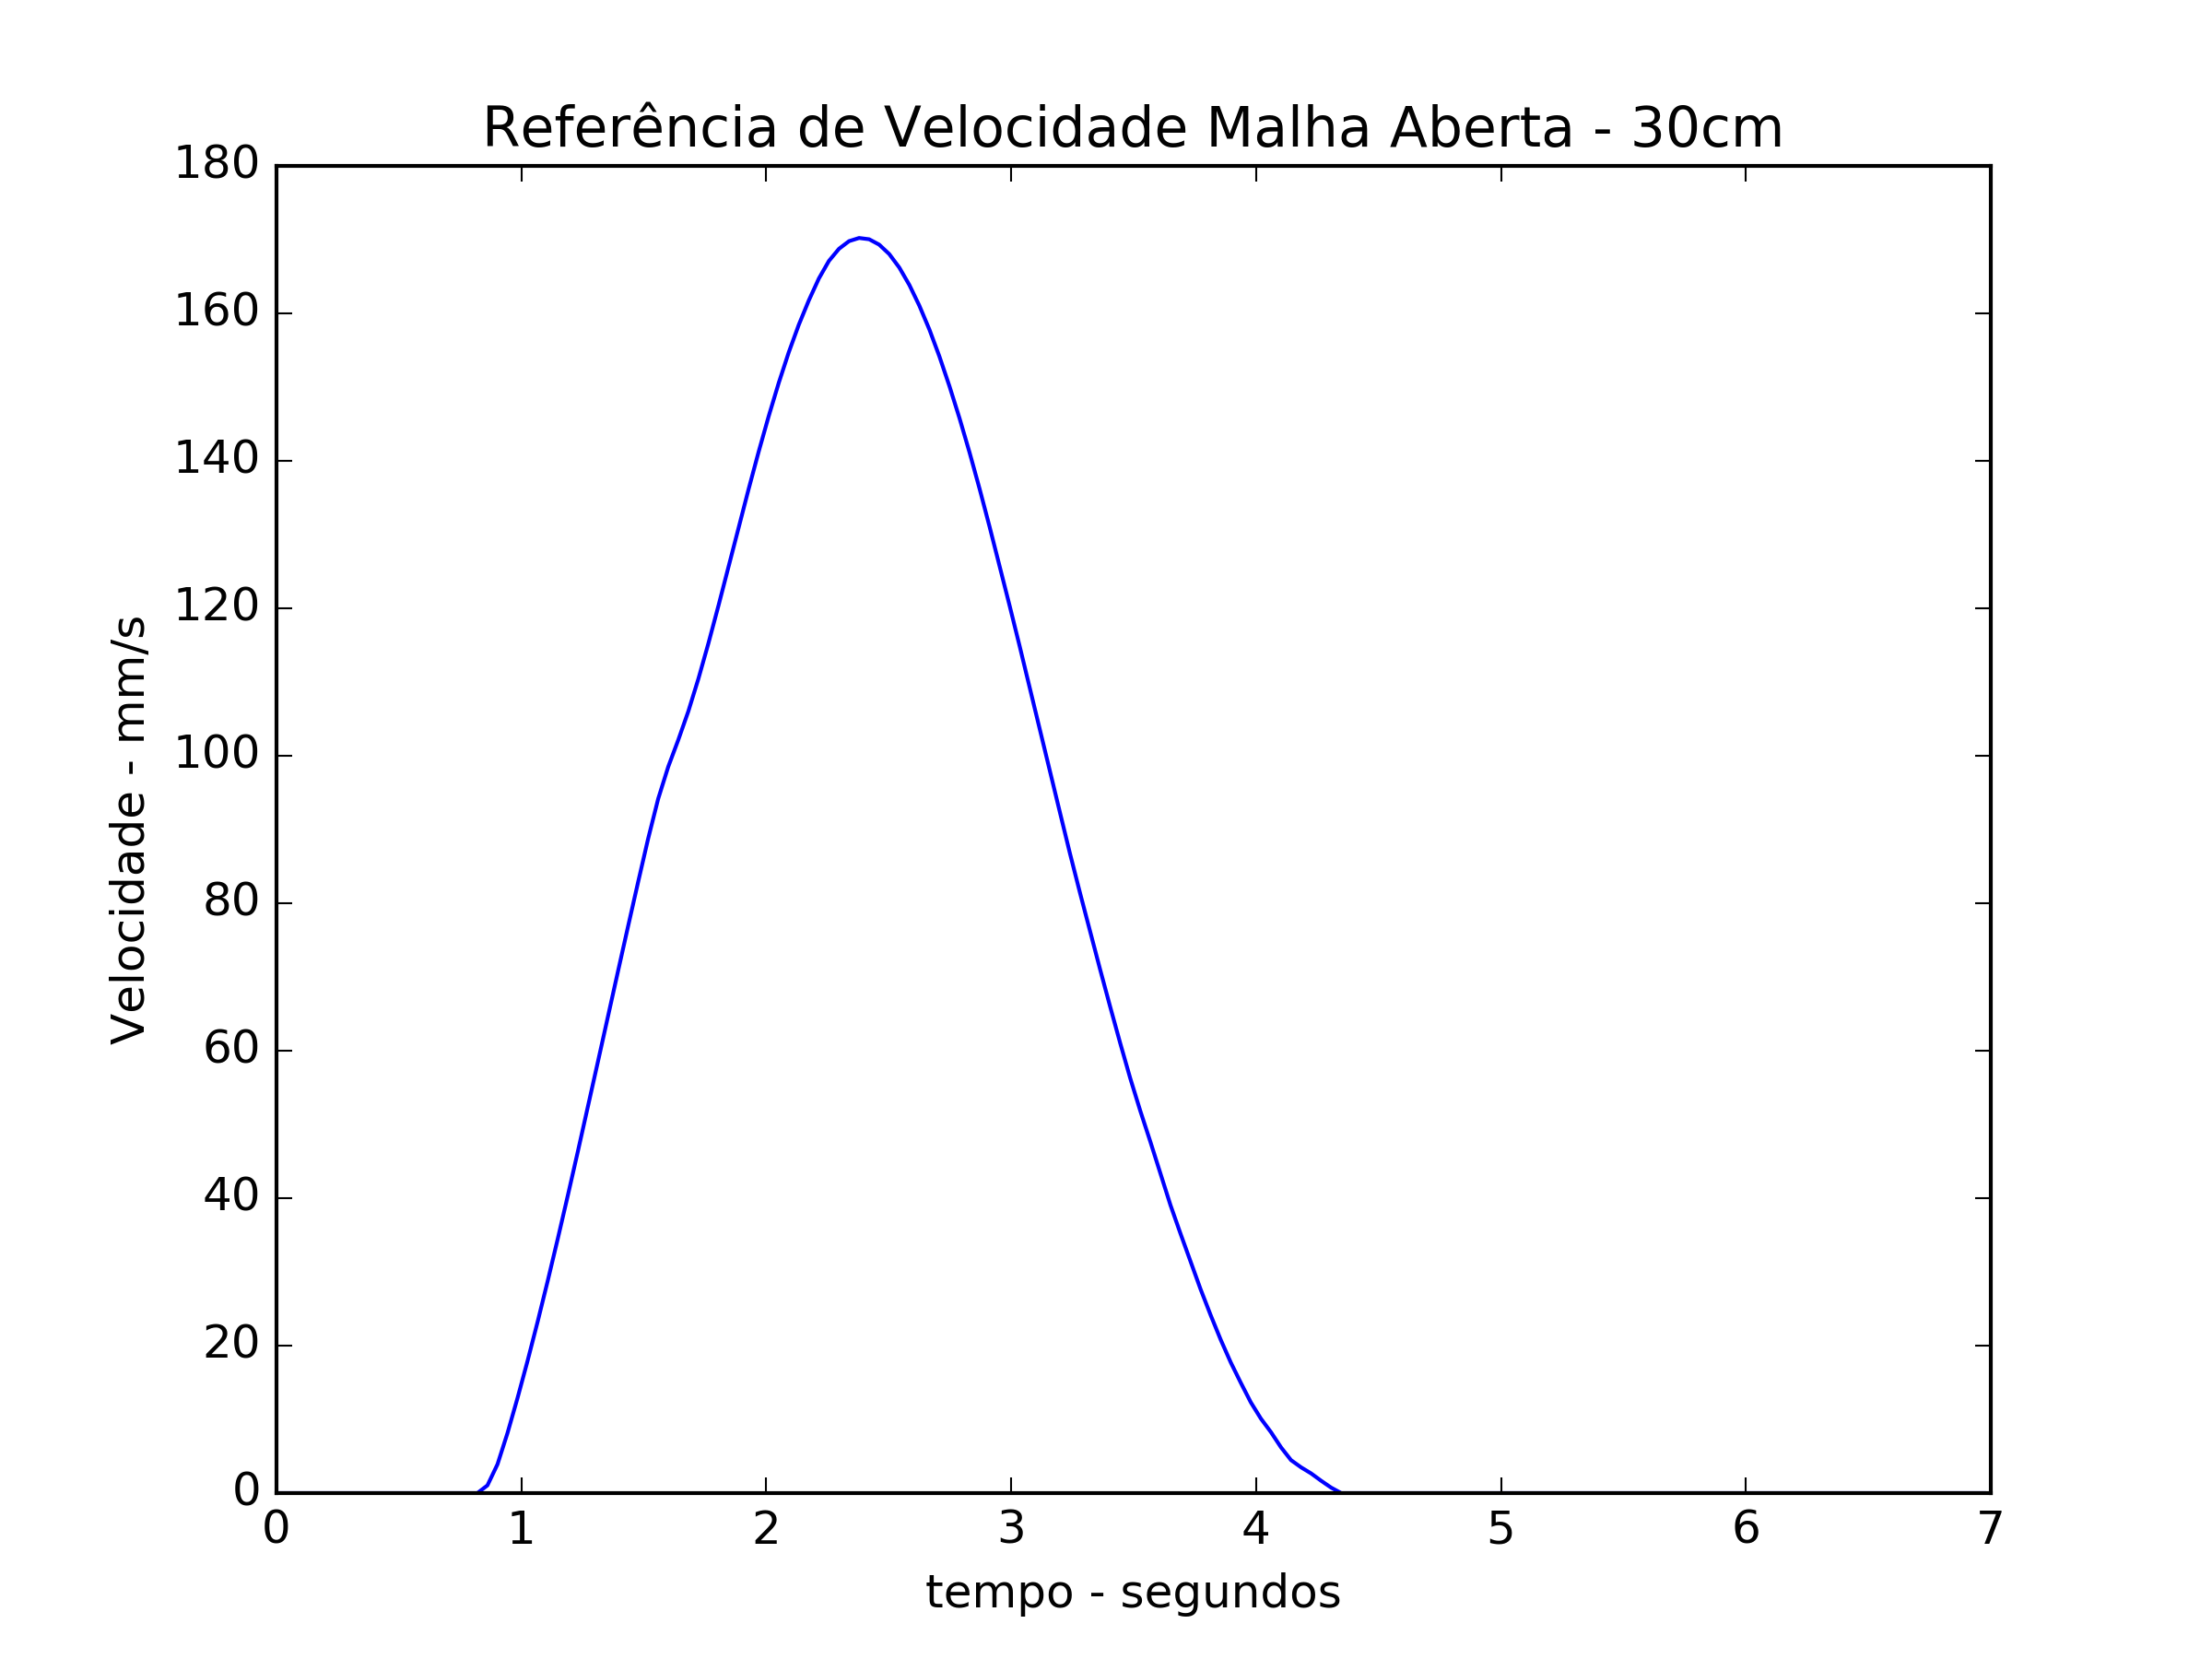
\includegraphics[width=1\linewidth]{figures/resultados/malha_aberta_1/VelocidadeT1}
        \caption{Referência de Velocidade para Excursão de 30cm}
        \label{VelocidadeT1}
    \end{minipage}
\end{figure}

\end{block}
\end{frame}

\begin{frame}[fragile]{Malha Aberta - Resultados}



\begin{block}{Excursão de 30 cm - Resultados}

\begin{figure}[!htb]
    \centering
    
    \begin{minipage}{.45\textwidth}
        \centering
        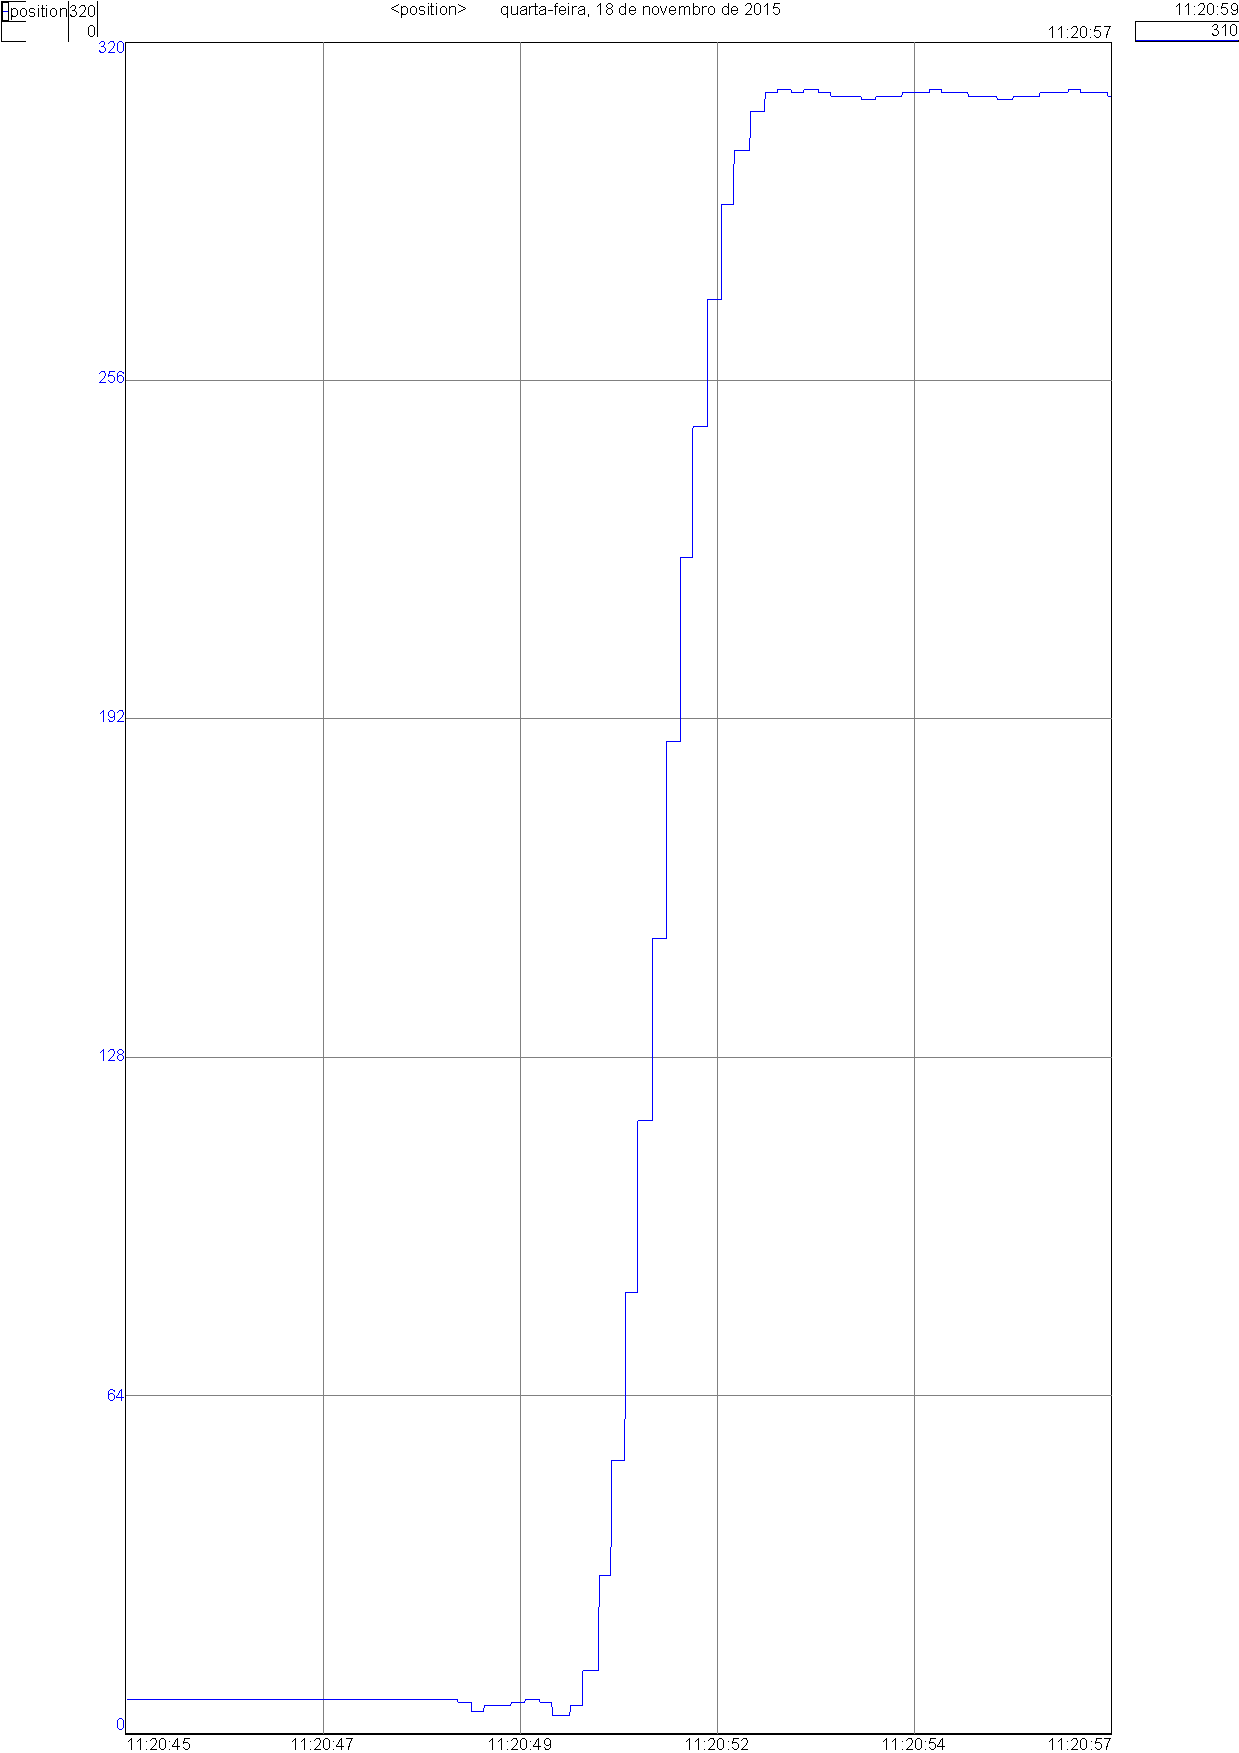
\includegraphics[width=\linewidth,height=4.5cm]{figures/resultados/malha_aberta_1/trajetoriaObtidaModelada.pdf}
        \caption{Resultado com Velocidade Modelada para Excursão de 30cm}
        \label{trajetoriaObtidaModelada}
    \end{minipage}%
    \hspace{0.1cm}
    \begin{minipage}{0.45\textwidth}
        \centering
        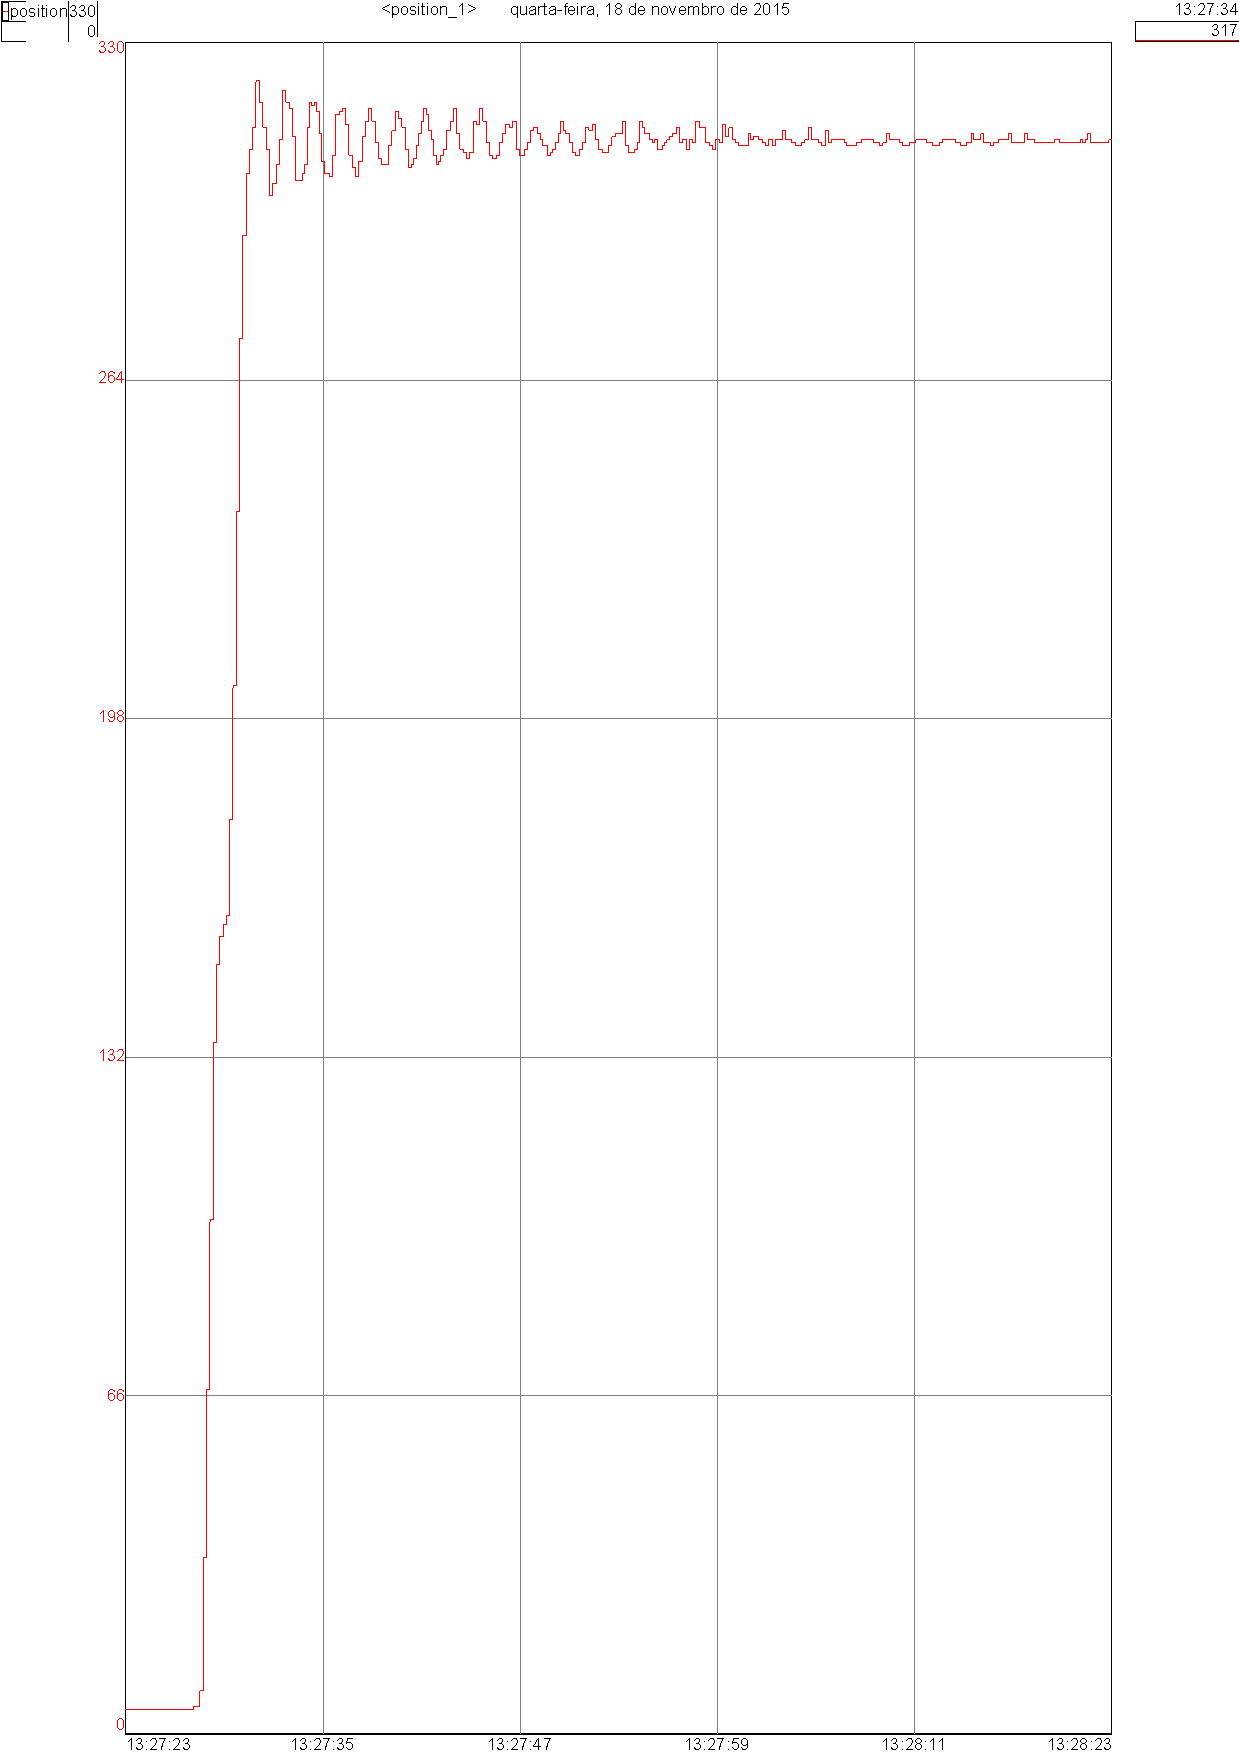
\includegraphics[width=1\linewidth,height=4.5cm]{figures/resultados/malha_aberta_1/trajetoriaObtidaVConstante.pdf}
        \caption{Resultado com Velocidade Constante para Excursão de 30cm}
        \label{trajetoriaObtidaVConstante}
    \end{minipage}
\end{figure}
\end{block}
\end{frame}

\begin{frame}[fragile]{Malha Aberta - Resultados}
\begin{block}{Excursão de 20 cm - Dados}
\begin{itemize}
	\item \textbf{Período de amostragem: } $T \approx 100 \mathrm{ms}$;
	\item \textbf{Deslocamento: } $\Delta x = 20 \mathrm{cm}$;
	\item \textbf{Intervalo de tempo: } $\Delta t \approx 1.5 \mathrm{s}$;
	\item \textbf{Velocidade média: } $\overline{v} = \frac{\Delta x}{\Delta t} \approx 133.3\mathrm{mm}/\mathrm{s}$.
	
\end{itemize}
\end{block}
\end{frame}

\begin{frame}[fragile]{Malha Aberta - Resultados}
\begin{block}{Excursão de 20 cm - Trajetória modelada}

\begin{figure}[!htb]
    \centering
    \begin{minipage}{.45\textwidth}
        \centering
        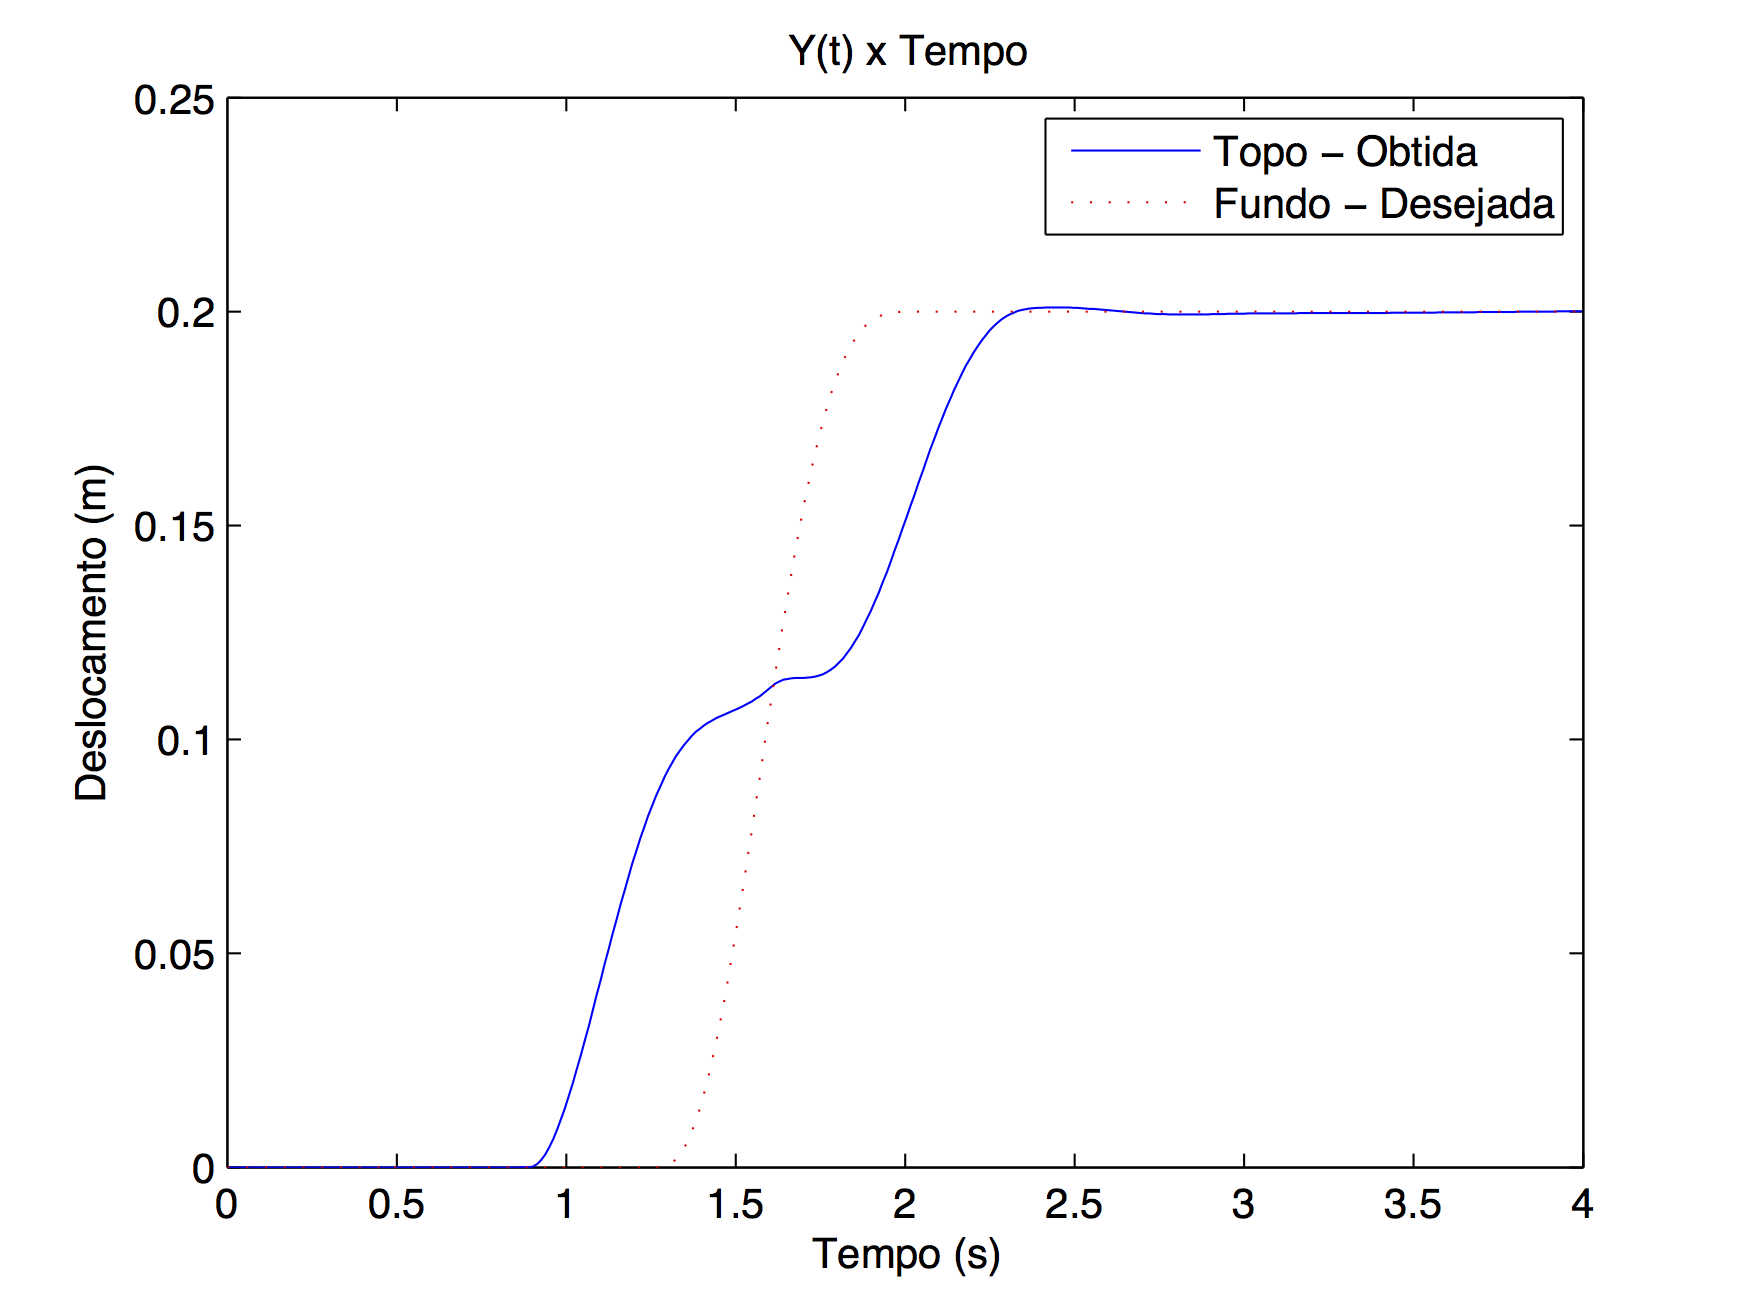
\includegraphics[width=1\linewidth]{figures/resultados/malha_aberta_2/DeslocamentoT2}
        \caption{Referência de Posição para Excursão de 20cm}
        \label{DeslocamentoT2}
    \end{minipage}%
    \hspace{0.1cm}
    \begin{minipage}{0.45\textwidth}
        \centering
        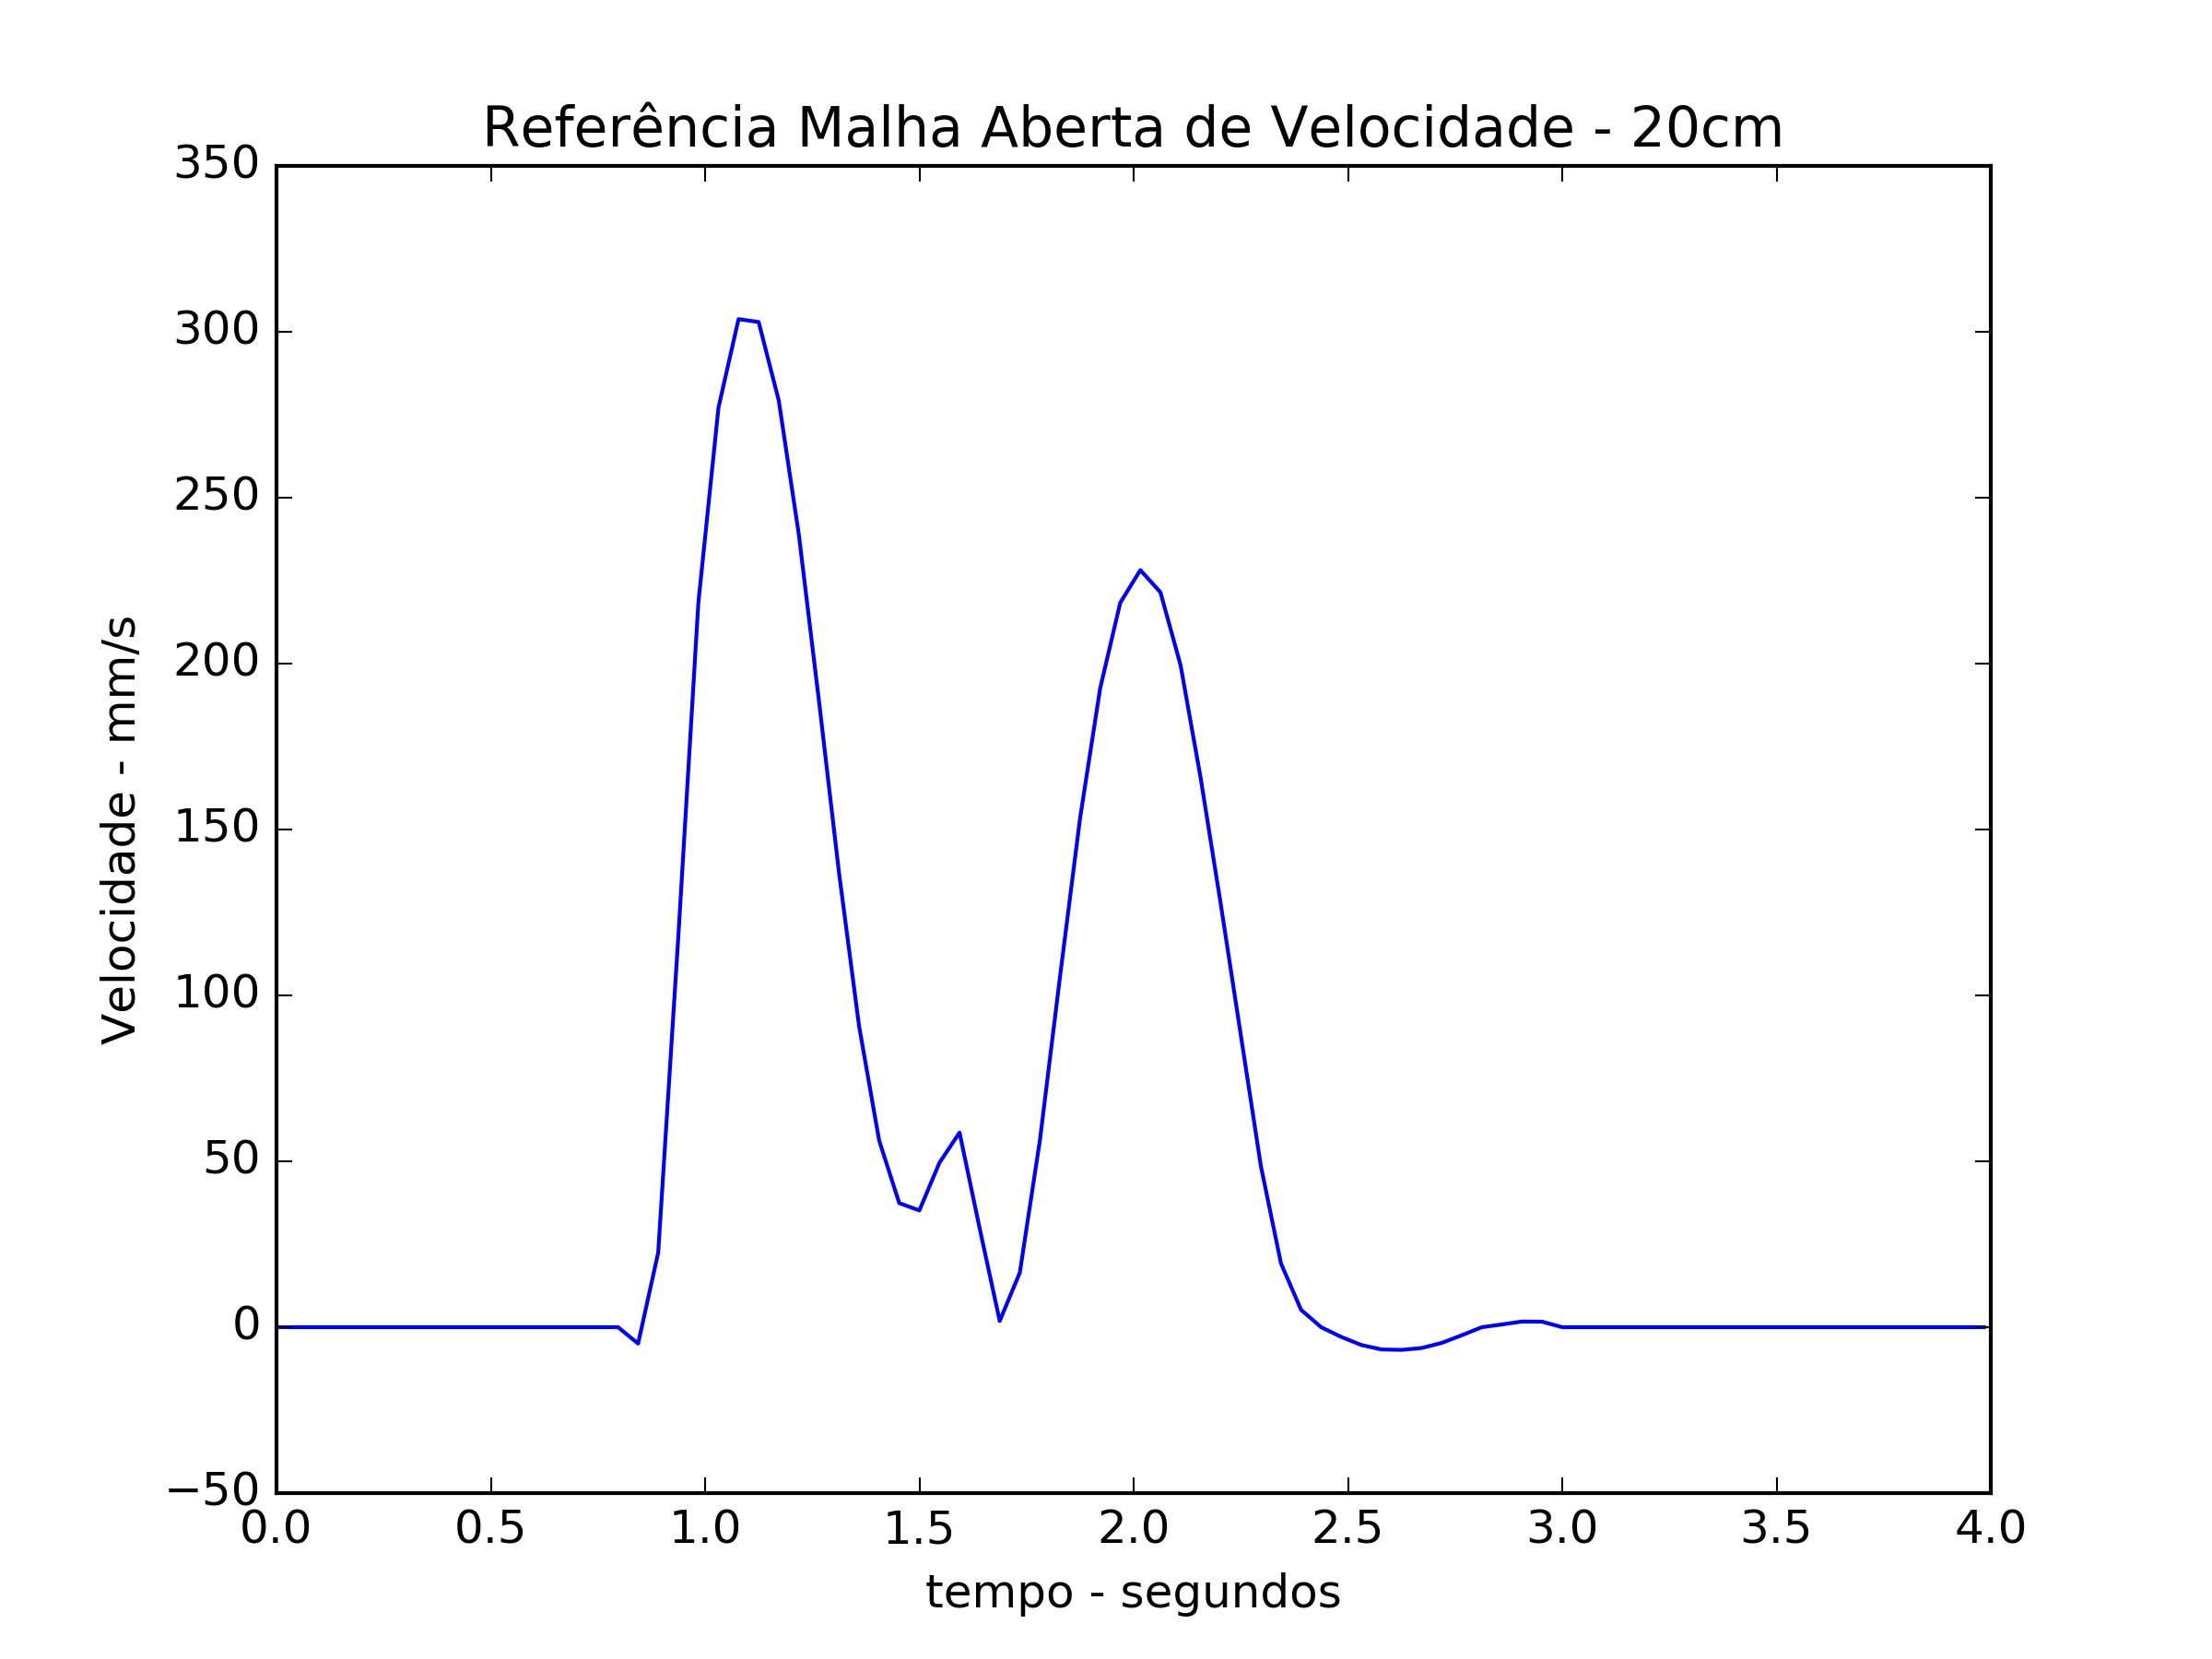
\includegraphics[width=1\linewidth]{figures/resultados/malha_aberta_2/VelocidadeT2}
        \caption{Referência de Velocidade para Excursão de 20cm}
        \label{VelocidadeT2}
    \end{minipage}
\end{figure}

\end{block}
\end{frame}

\begin{frame}[fragile]{Malha Aberta - Resultados}

\begin{block}{Excursão de 20 cm - Resultados}

\begin{figure}[!htb]
    \centering
    \begin{minipage}{.45\textwidth}
        \centering
        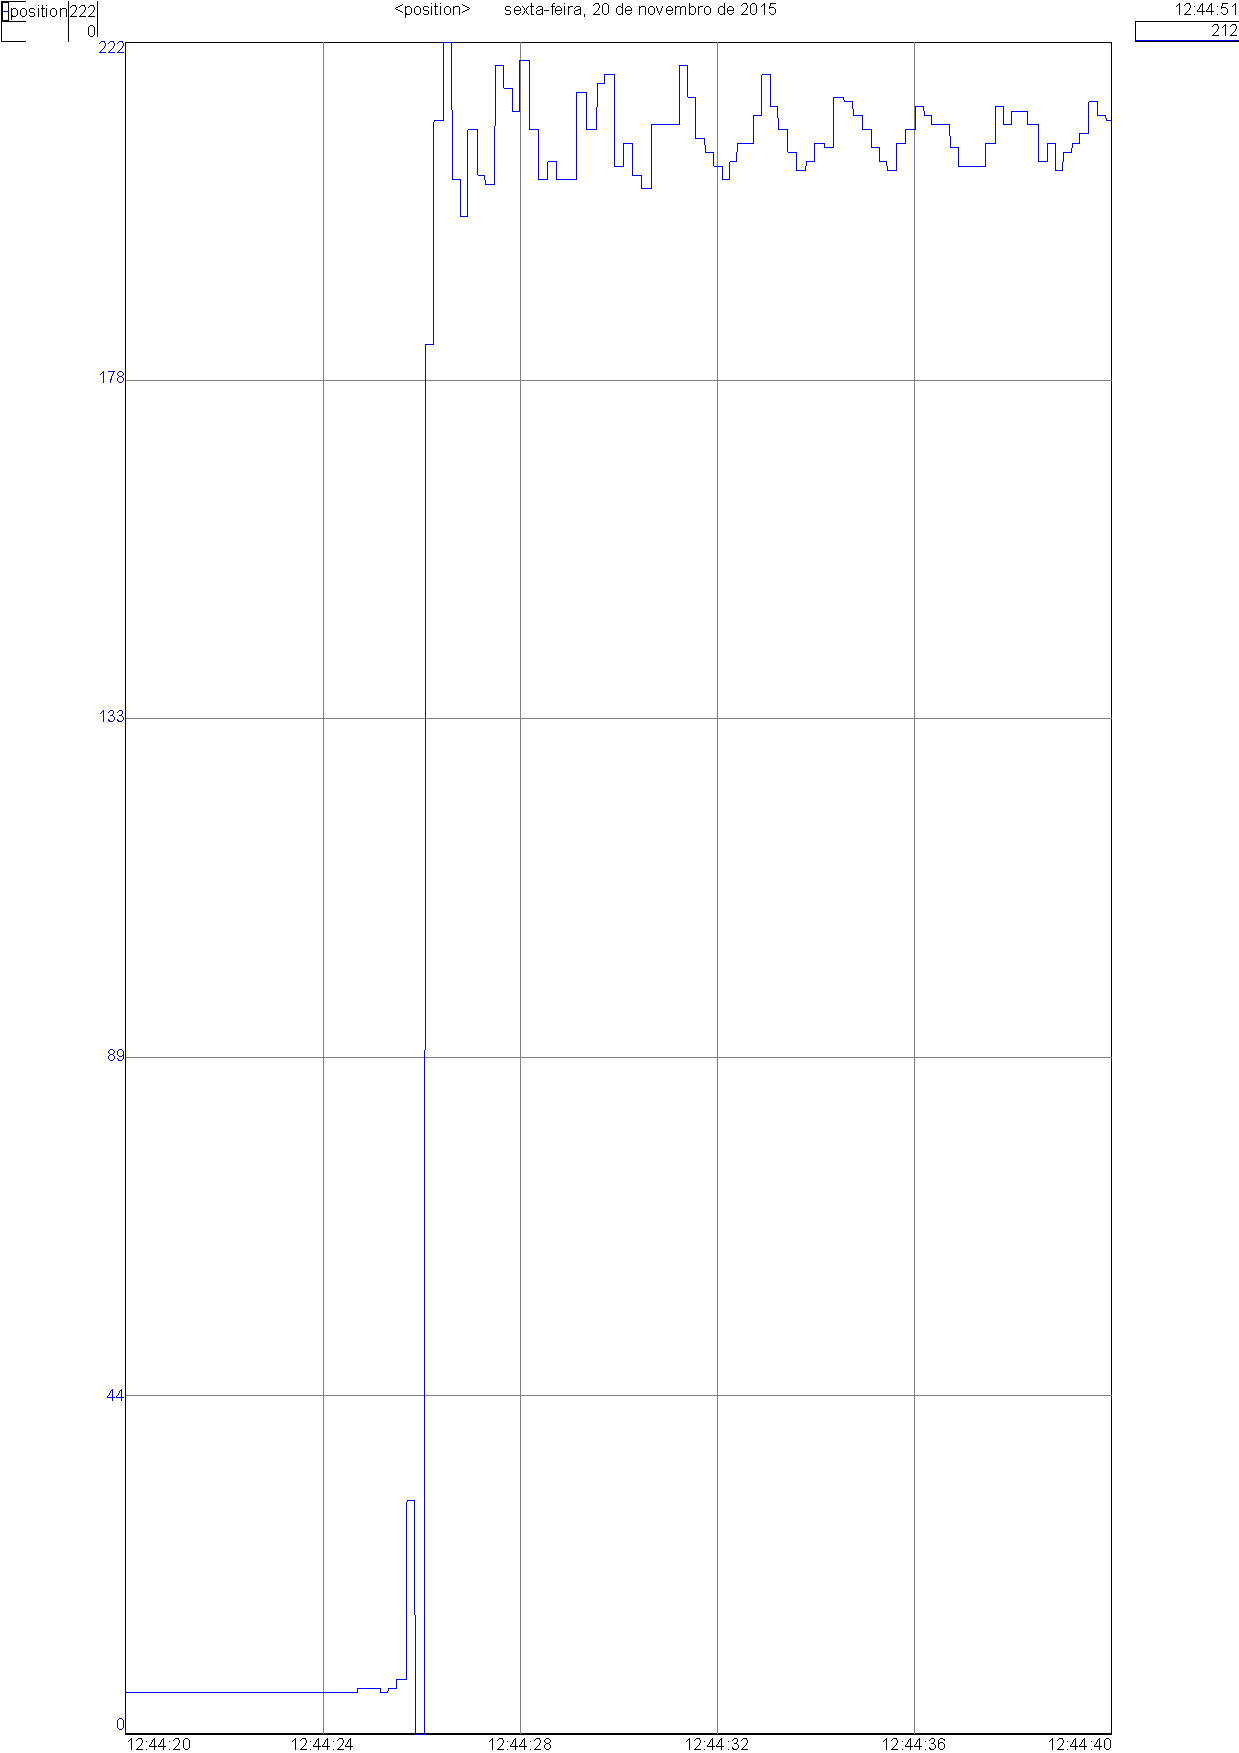
\includegraphics[width=1\linewidth,height=4.5cm]{figures/resultados/malha_aberta_2/percurso20cmBom.pdf}
        \caption{Resultado com Velocidade Modelada para Excursão de 20cm}
        \label{percurso20cmBom}
    \end{minipage}%
    \hspace{0.1cm}
    \begin{minipage}{0.45\textwidth}
        \centering
        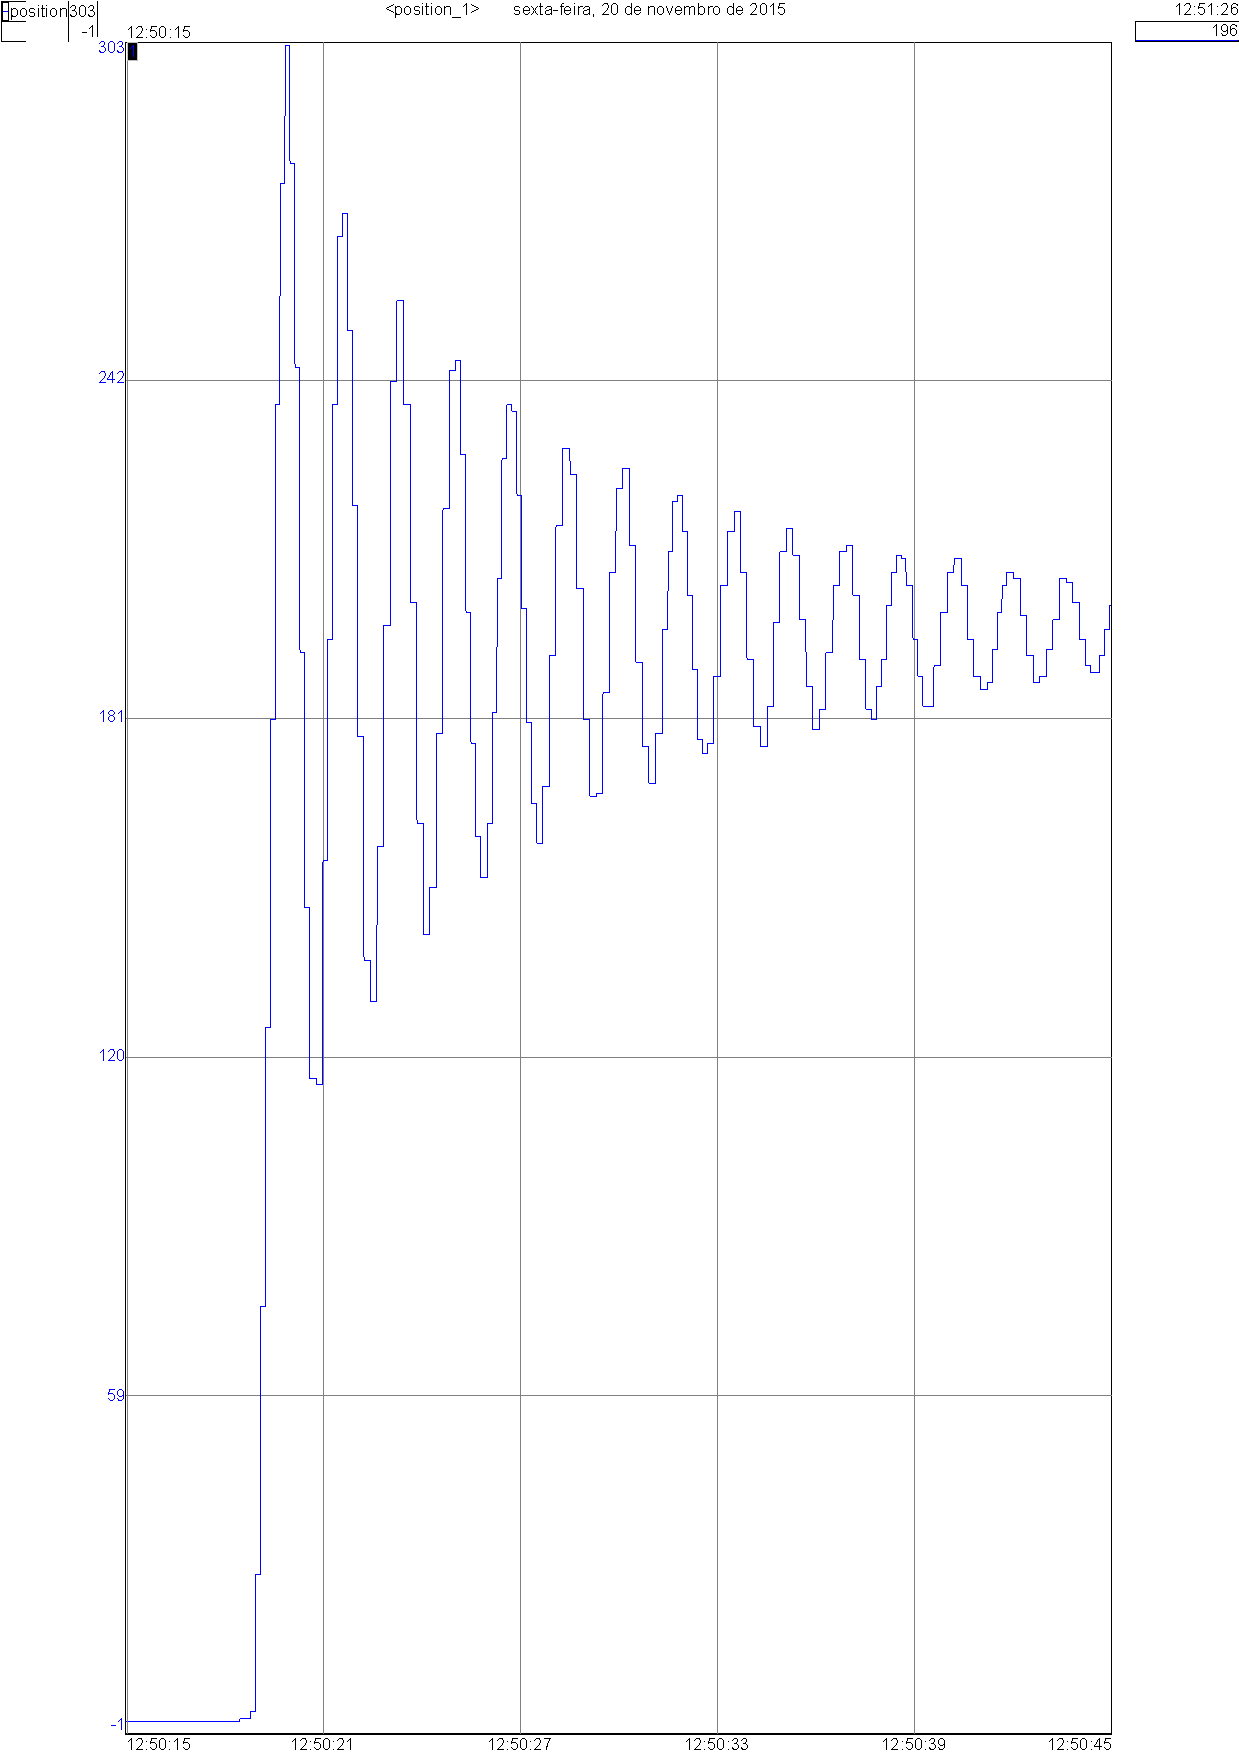
\includegraphics[width=1\linewidth,height=4.5cm]{figures/resultados/malha_aberta_2/percurso20cmRuim.pdf}
        \caption{Resultado com Velocidade Constante para Excursão de 20cm}
        \label{percurso20cmRuim}
    \end{minipage}
\end{figure}
\end{block}
\end{frame}

\begin{frame}[fragile]{Malha Fechada - Resultados}
\begin{block}{Controlador P - Ensaios}
Foram feitos dois ensaios:
\begin{enumerate}
	\item $K_p = 0.0050 \frac{\mathrm{u}}{\mathrm{mm}\cdot\mathrm{s}}$;
	\item $K_p = 0.0025 \frac{\mathrm{u}}{\mathrm{mm}\cdot\mathrm{s}}$.
\end{enumerate}
\end{block}
\end{frame}

\begin{frame}[fragile]{Malha Fechada - Resultados}

\tikzstyle{block} = [draw, fill=blue!20, rectangle,
minimum height=3em, minimum width=6em]
\tikzstyle{sum} = [draw, fill=blue!20, circle, node distance=1cm]
\tikzstyle{input} = [coordinate]
\tikzstyle{output} = [coordinate]
\tikzstyle{pinstyle} = [pin edge={to-,thin,black}]

\begin{block}{Controlador P - Esquemático}
\begin{figure}[!ht]
\centering
\begin{tikzpicture}[auto, node distance=2cm,>=latex']
% We start by placing the blocks
\node [input, name=input] {};
\node [sum, right of=input] (sum) {};
\node [block, right of=sum] (controller) {$K_p$};
\node [block, right of=controller, pin={[pinstyle]above:Perturbações},
node distance=3cm] (system) {Planta};
% We draw an edge between the controller and system block to 
% calculate the coordinate u. We need it to place the measurement block. 
\draw [->] (controller) -- node[name=u] {$v$} (system);
\node [output, right of=system] (output) {};
\node [block, below of=u] (measurements) {Câmera};

% Once the nodes are placed, connecting them is easy. 
\draw [draw,->] (input) -- node {$r$} (sum);
\draw [->] (sum) -- node {$e$} (controller);
\draw [->] (system) -- node [name=y] {$y$}(output);
\draw [->] (y) |- (measurements);
\draw [->] (measurements) -| node[pos=0.99] {$-$} 
node [near end] {$y_m$} (sum);
\end{tikzpicture}
\caption{Malha fechada de controle\label{mfechadaP}}
\end{figure}
\end{block}
\end{frame}

\begin{frame}[fragile]{Malha Fechada - Resultados}
\begin{block}{Controlador P - Resultados}
\begin{figure}[!htb]
    \centering
    \begin{minipage}{.45\textwidth}
        \centering
        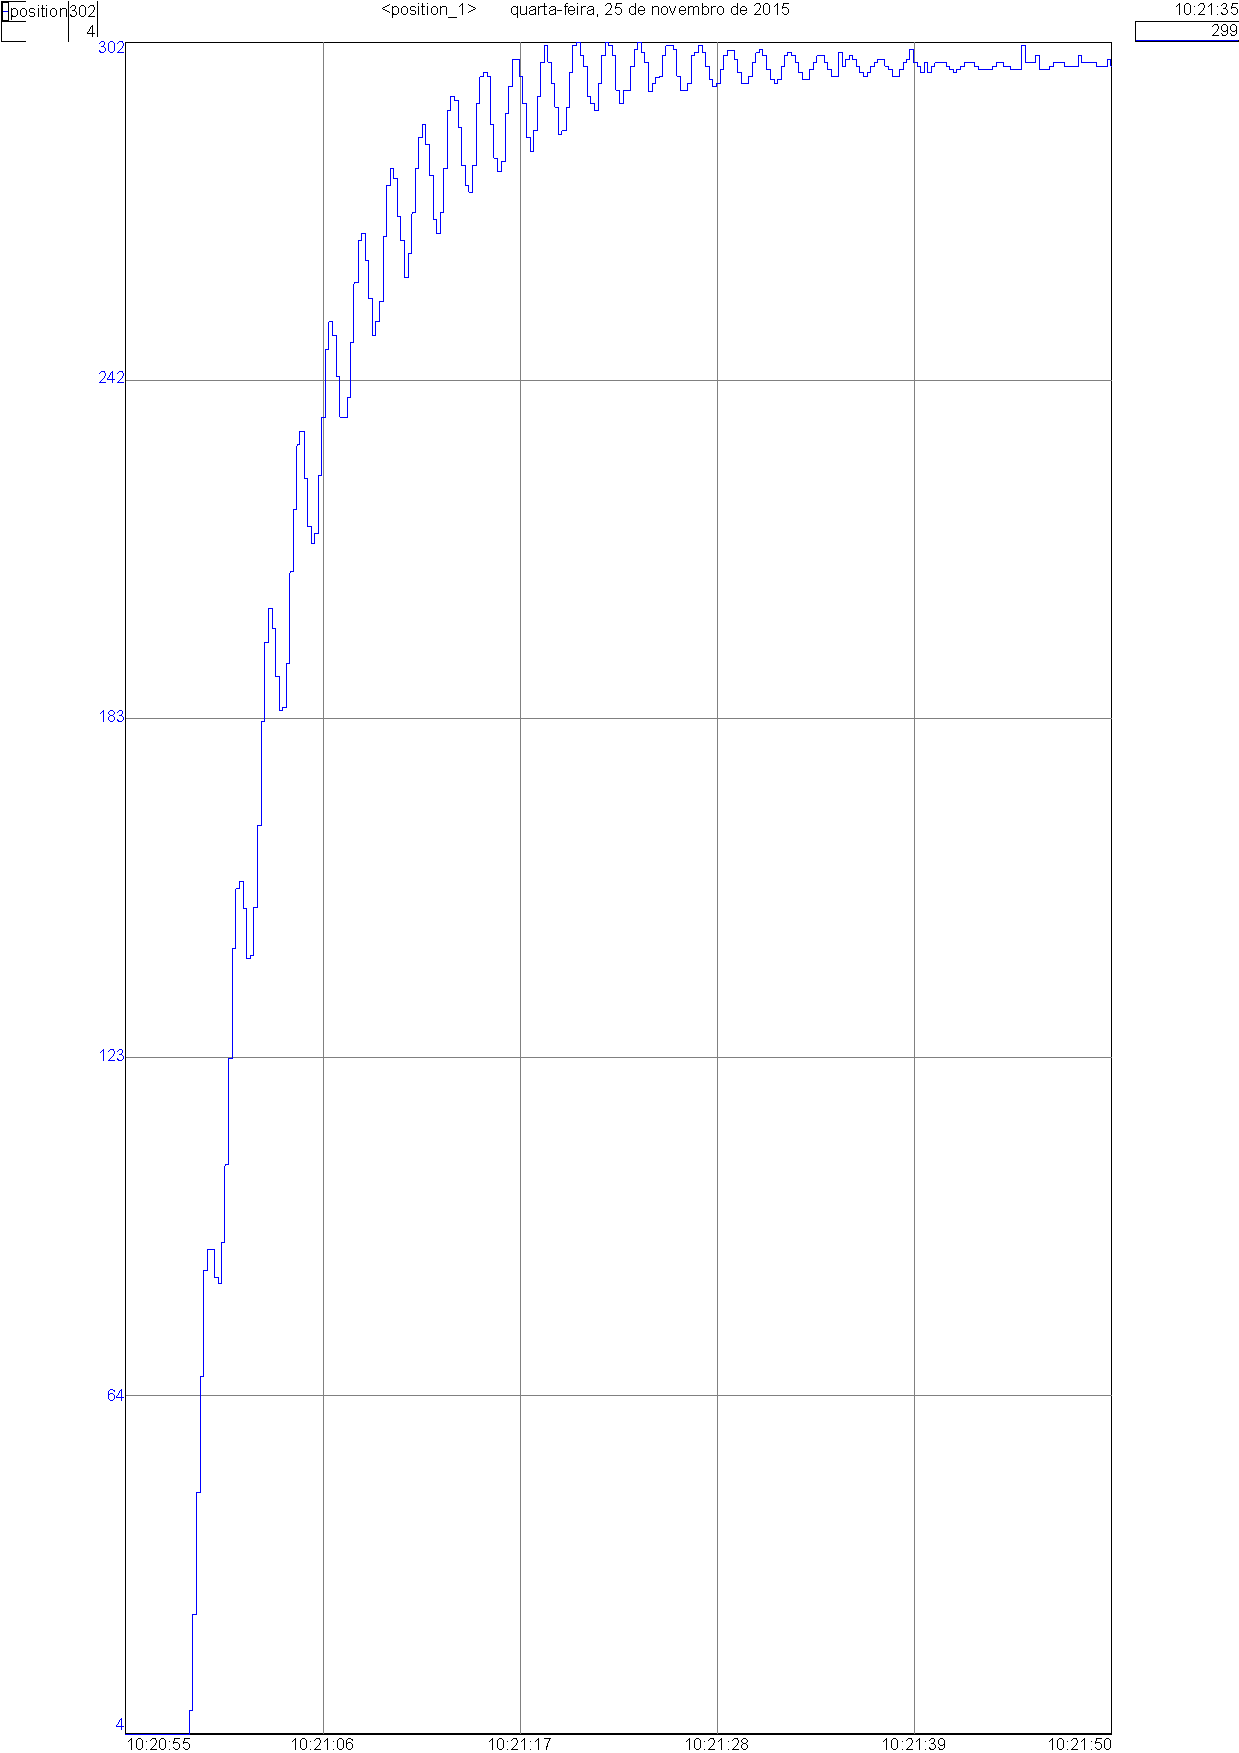
\includegraphics[width=1\linewidth,height=4.5cm]{figures/resultados/malha_fechada_P/MF_Proporcional_Kp_00025.pdf}
        \caption{Resultado com Malha Fechada Proporcional e $K_p = 0.0025\frac{\mathrm{u}}{\mathrm{mm}\cdot\mathrm{s}}$}
        \label{MFProporcionalKpbaixo}
    \end{minipage}%
    \hspace{0.1cm}
    \begin{minipage}{0.45\textwidth}
        \centering
        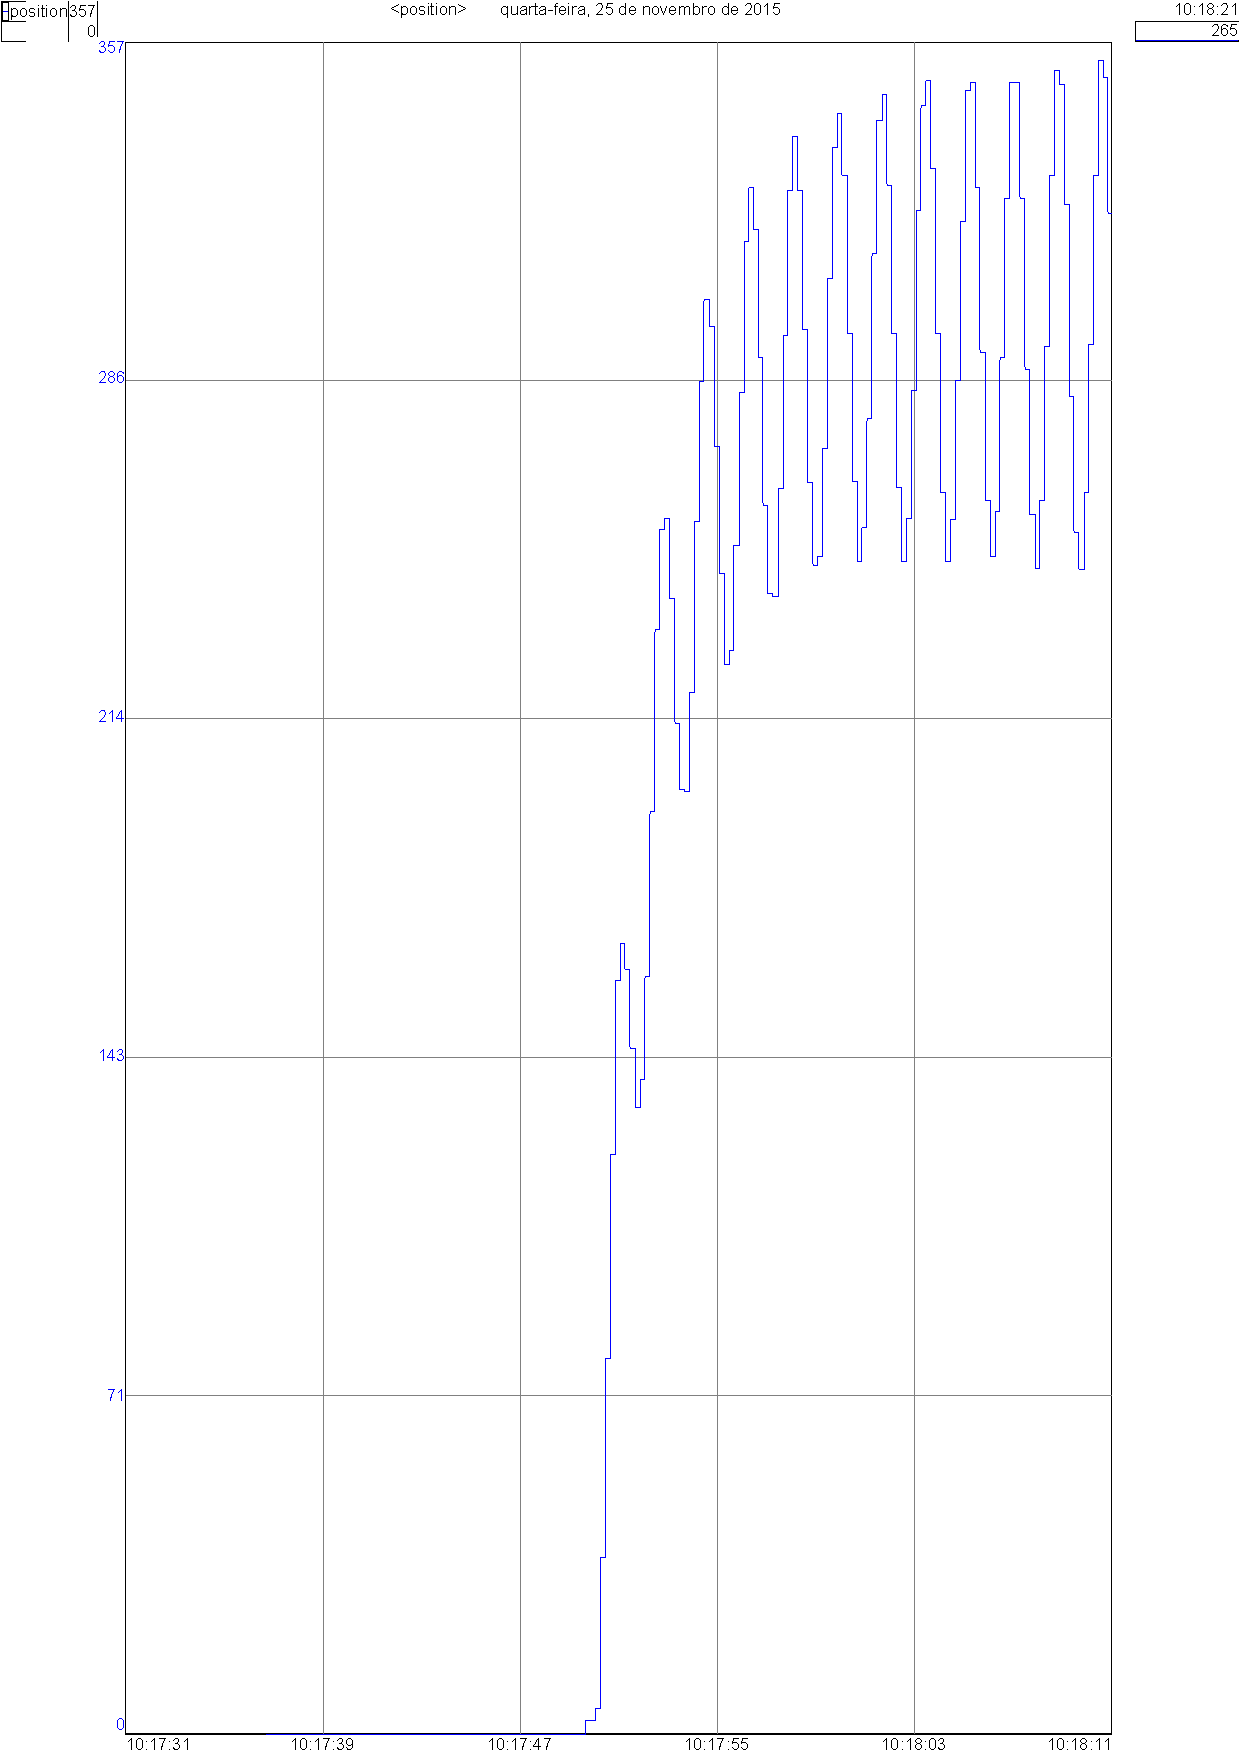
\includegraphics[width=1\linewidth,height=4.5cm]{figures/resultados/malha_fechada_P/MF_Proporcional_Kp_00050.pdf}
        \caption{Resultado com Malha Fechada Proporcional e $K_p = 0.0050\frac{\mathrm{u}}{\mathrm{mm}\cdot\mathrm{s}}$
        \label{MFProporcionalKpmedio}}
    \end{minipage}
\end{figure}
\end{block}
\end{frame}

\begin{frame}[fragile]{\textit{Links} Interessantes}
\begin{block}{\textit{Links} para vídeos com resultados}
\begin{enumerate}
	\item Excursão 30 cm (1) - \url{https://youtu.be/lKajz6LyauE}
	\item Excursão 30 cm (2) - \url{https://youtu.be/tB0TsmBcfVg}
	\item Excursão 20 cm (1) - \url{https://youtu.be/wg1Wq_6VRSg}
	\item Excursão 20 cm (2) - \url{https://youtu.be/Ges2-eYy69k}
	\item Controlador P com $K_p = 0.0050$ - \url{https://youtu.be/sHh3yvBrek4} 
	\item Controlador P com $K_p = 0.0025$ - \url{https://youtu.be/mmT1ZwFBJ4s}
\end{enumerate}
\end{block}
\end{frame}
%\begin{frame}[fragile]{Typography}
%      \begin{verbatim}The theme provides sensible defaults to
%\emph{emphasize} text, \alert{accent} parts
%or show \textbf{bold} results.\end{verbatim}
%
%  \begin{center}becomes\end{center}
%
%  The theme provides sensible defaults to \emph{emphasize} text,
%  \alert{accent} parts or show \textbf{bold} results.
%\end{frame}
%
%\begin{frame}{Font feature test}
%  \begin{itemize}
%    \item Regular
%    \item \textit{Italic}
%    \item \textsc{SmallCaps}
%    \item \textbf{Bold}
%    \item \textbf{\textit{Bold Italic}}
%    \item \textbf{\textsc{Bold SmallCaps}}
%    \item \texttt{Monospace}
%    \item \texttt{\textit{Monospace Italic}}
%    \item \texttt{\textbf{Monospace Bold}}
%    \item \texttt{\textbf{\textit{Monospace Bold Italic}}}
%  \end{itemize}
%\end{frame}
%
%\begin{frame}{Lists}
%  \begin{columns}[T,onlytextwidth]
%    \column{0.33\textwidth}
%      Items
%      \begin{itemize}
%        \item Milk \item Eggs \item Potatos
%      \end{itemize}
%
%    \column{0.33\textwidth}
%      Enumerations
%      \begin{enumerate}
%        \item First, \item Second and \item Last.
%      \end{enumerate}
%
%    \column{0.33\textwidth}
%      Descriptions
%      \begin{description}
%        \item[PowerPoint] Meeh. \item[Beamer] Yeeeha.
%      \end{description}
%  \end{columns}
%\end{frame}
%\begin{frame}{Animation}
%  \begin{itemize}[<+- | alert@+>]
%    \item \alert<4>{This is\only<4>{ really} important}
%    \item Now this
%    \item And now this
%  \end{itemize}
%\end{frame}
%\begin{frame}{Figures}
%  \begin{figure}
%    \newcounter{density}
%    \setcounter{density}{20}
%    \begin{tikzpicture}
%      \def\couleur{alerted text.fg}
%      \path[coordinate] (0,0)  coordinate(A)
%                  ++( 90:5cm) coordinate(B)
%                  ++(0:5cm) coordinate(C)
%                  ++(-90:5cm) coordinate(D);
%      \draw[fill=\couleur!\thedensity] (A) -- (B) -- (C) --(D) -- cycle;
%      \foreach \x in {1,...,40}{%
%          \pgfmathsetcounter{density}{\thedensity+20}
%          \setcounter{density}{\thedensity}
%          \path[coordinate] coordinate(X) at (A){};
%          \path[coordinate] (A) -- (B) coordinate[pos=.10](A)
%                              -- (C) coordinate[pos=.10](B)
%                              -- (D) coordinate[pos=.10](C)
%                              -- (X) coordinate[pos=.10](D);
%          \draw[fill=\couleur!\thedensity] (A)--(B)--(C)-- (D) -- cycle;
%      }
%    \end{tikzpicture}
%    \caption{Rotated square from
%    \href{http://www.texample.net/tikz/examples/rotated-polygons/}{texample.net}.}
%  \end{figure}
%\end{frame}
%\begin{frame}{Tables}
%  \begin{table}
%    \caption{Largest cities in the world (source: Wikipedia)}
%    \begin{tabular}{lr}
%      \toprule
%      City & Population\\
%      \midrule
%      Mexico City & 20,116,842\\
%      Shanghai & 19,210,000\\
%      Peking & 15,796,450\\
%      Istanbul & 14,160,467\\
%      \bottomrule
%    \end{tabular}
%  \end{table}
%\end{frame}
%\begin{frame}{Blocks}
%  Three different block environments are pre-defined and may be styled with an
%  optional background color.
%
%  \begin{columns}[T,onlytextwidth]
%    \column{0.5\textwidth}
%      \begin{block}{Default}
%        Block content.
%      \end{block}
%
%      \begin{alertblock}{Alert}
%        Block content.
%      \end{alertblock}
%
%      \begin{exampleblock}{Example}
%        Block content.
%      \end{exampleblock}
%
%    \column{0.5\textwidth}
%
%      \metroset{block=fill}
%
%      \begin{block}{Default}
%        Block content.
%      \end{block}
%
%      \begin{alertblock}{Alert}
%        Block content.
%      \end{alertblock}
%
%      \begin{exampleblock}{Example}
%        Block content.
%      \end{exampleblock}
%
%  \end{columns}
%\end{frame}
%\begin{frame}{Math}
%  \begin{equation*}
%    e = \lim_{n\to \infty} \left(1 + \frac{1}{n}\right)^n
%  \end{equation*}
%\end{frame}
%\begin{frame}{Line plots}
%  \begin{figure}
%    \begin{tikzpicture}
%      \begin{axis}[
%        mlineplot,
%        width=0.9\textwidth,
%        height=6cm,
%      ]
%
%        \addplot {sin(deg(x))};
%        \addplot+[samples=100] {sin(deg(2*x))};
%
%      \end{axis}
%    \end{tikzpicture}
%  \end{figure}
%\end{frame}
%\begin{frame}{Bar charts}
%  \begin{figure}
%    \begin{tikzpicture}
%      \begin{axis}[
%        mbarplot,
%        xlabel={Foo},
%        ylabel={Bar},
%        width=0.9\textwidth,
%        height=6cm,
%      ]
%
%      \addplot plot coordinates {(1, 20) (2, 25) (3, 22.4) (4, 12.4)};
%      \addplot plot coordinates {(1, 18) (2, 24) (3, 23.5) (4, 13.2)};
%      \addplot plot coordinates {(1, 10) (2, 19) (3, 25) (4, 15.2)};
%
%      \legend{lorem, ipsum, dolor}
%
%      \end{axis}
%    \end{tikzpicture}
%  \end{figure}
%\end{frame}
%\begin{frame}{Quotes}
%  \begin{quote}
%    Veni, Vidi, Vici
%  \end{quote}
%\end{frame}
%
%\begin{frame}{References}
%  Some references to showcase [allowframebreaks] \cite{knuth92,ConcreteMath,Simpson,Er01,greenwade93}
%\end{frame}

\section{Conclusão}

\begin{frame}[fragile]{Conclusão}
\begin{block}{Conclusões}
\begin{itemize}
	\item Adquiriu-se um conhecimento relativamente alto da bancada em que foi realizado o experimento;
	\item Foi possível fechar a malha de controle, ainda que fosse um controlador P, cujo resultado não é ideal.
\end{itemize}
\end{block}
\end{frame}

\begin{frame}[fragile]{Conclusão}
\begin{block}{Perspectivas Futuras}
\begin{itemize}
	\item Utilizar uma abordagem de controle mais rebuscada, utilizando redução modal, conforme Fabrício et al \cite{fabricioIFAC};
	\item Buscar soluções envolvendo controle preditivo, de forma a se obter melhores resultados.
\end{itemize}
\end{block}
\end{frame}

%\begin{frame}{Summary}
%
%  Get the source of this theme and the demo presentation from
%
%  \begin{center}\url{github.com/matze/mtheme}\end{center}
%
%  The theme \emph{itself} is licensed under a
%  \href{http://creativecommons.org/licenses/by-sa/4.0/}{Creative Commons
%  Attribution-ShareAlike 4.0 International License}.
%
%  \begin{center}\ccbysa\end{center}
%
%\end{frame}

\plain{Dúvidas?}

\begin{frame}[allowframebreaks]{Referências}

  \bibliography{apresentacaoTG2}
  \bibliographystyle{abbrv}

\end{frame}

\plain{Obrigado!}

\end{document}
